
\documentclass[review]{elsarticle}

\usepackage{lineno,hyperref}
\usepackage[mathletters]{ucs}
\usepackage[utf8x]{inputenc}
\usepackage[linesnumbered, ruled, vlined]{algorithm2e}
\usepackage{natbib}
\usepackage{supertabular}
\usepackage{fancybox}
\usepackage{acronym}
\usepackage{array}
\usepackage{booktabs}
\usepackage{graphicx}
\usepackage{rotating}
\usepackage{tabularx}
\usepackage{multirow}
\usepackage{hhline}
\usepackage{setspace}
\usepackage{placeins}
\usepackage{longtable}
\usepackage{listings}
\usepackage{epstopdf}
\usepackage{subfigure}
\usepackage{courier}
\usepackage{amsfonts}
\usepackage{morefloats}
\usepackage{lipsum}
\usepackage{mathtools}
\usepackage{amsthm,amsmath}

% table
\usepackage{makecell}
\usepackage{color, colortbl}
\definecolor{Gray}{gray}{0.9}

% appendix
\usepackage[titletoc,title]{appendix}
\usepackage{hyperref}
\usepackage{cleveref}

% norm


\modulolinenumbers[5]

\journal{Journal of Network and Computer Applications}

%%%%%%%%%%%%%%%%%%%%%%%
%% Elsevier bibliography styles
%%%%%%%%%%%%%%%%%%%%%%%
%% To change the style, put a % in front of the second line of the current style and
%% remove the % from the second line of the style you would like to use.
%%%%%%%%%%%%%%%%%%%%%%%

%% Numbered
%\bibliographystyle{model1-num-names}

%% Numbered without titles
%\bibliographystyle{model1a-num-names}

%% Harvard
%\bibliographystyle{model2-names.bst}\biboptions{authoryear}

%% Vancouver numbered
%\usepackage{numcompress}\bibliographystyle{model3-num-names}

%% Vancouver name/year
%\usepackage{numcompress}\bibliographystyle{model4-names}\biboptions{authoryear}

%% APA style
%\bibliographystyle{model5-names}\biboptions{authoryear}

%% AMA style
%\usepackage{numcompress}\bibliographystyle{model6-num-names}

%% `Elsevier LaTeX' style
\bibliographystyle{elsarticle-num}
%%%%%%%%%%%%%%%%%%%%%%%

\begin{document}

\begin{frontmatter}

\title{Moment Distances from Robust Subspace for Botnet Detection}

%% Group authors per affiliation:
\author[unbaddress]{Thiago P. B. Vieira}
\author[unbaddress]{Eduardo S. C. Vilaça}
\author[unbaddress,Ilmenauaddress,Fraunhoferaddress]{João Paulo C. L. da Costa}
\author[unbaddress]{Éder S. Gualberto}
\author[unbaddress]{Rafael T. de Sousa Júnior}

\address[unbaddress]{Department of Electrical Engineering, University of Brasilia (UnB), 70910-900, Brasília-DF, Brazil}
\address[Ilmenauaddress]{Institute for Information Technology, Ilmenau University of Technology, Ilmenau, Germany}
\address[Fraunhoferaddress]{Fraunhofer Institute for Integrated Circuits IIS, Erlangen, Germany}


\begin{abstract}
The U.S. government estimates that malicious cyber activity cost the U.S. economy between US\$57 billion and US\$109 billion in 2016. Accenture argues that 89\% of survey respondents believe breakthrough technologies, like artificial intelligence, machine learning and user behavior analytics, are essential for securing organizations. The imbalanced data can compromise the performance of standard learning algorithms, creating bias or unfair weight to learn from the majority class and reducing detection capacity of anomalies. Some widely adopted algorithms for anomaly detection assume a Gaussian distributed data for legitimate observations, but this assumption may not be observed in network traffic, which is usually characterized by skewed and heavy-tailed distributions. We propose the Moment-based Robust Principal Component Analysis (m-RPCA) for botnet attack detection, which is a framework based on distances between contaminated observations and moments computed from a robust subspace learned by RPCA, to detect anomalies and network attacks. We evaluate m-RPCA on simulated data and on CTU-13 data set, and results show that m-RPCA can improve the botnet attack detection and the anomaly detection on skewed data, in comparison to anomaly detection algorithms.
\end{abstract}

\begin{keyword}
Anomaly Detection, Botnet Attack Detection, Skewed Data, Imbalanced Data, Robust Principal Component Analysis (RPCA).
\end{keyword}

\end{frontmatter}

\linenumbers

%%%%%%%%%%%%%%%%%%%%%%%%%%%%%%%%%%%%%%%%%%%%%%%%%%%%%%%%%%%%%%%%%%%%%%%%%%%%%%%%%%%%%%%%%%%%%%%%%%%%%%%%%%%%%%%%%%%%%%%%%%%%%%%%%%%%%%%%%%%%%%%%%%%%%%%%%%%%%%%%%%%%%%%%%%%%%%%%%%%%%%%%%%%%%%%%%%%%%%%%%%%%%%%%%%%%%%%%%%%%
\section{Introduction}
\label{sec:introduction}


According to \cite{distilnetworks2019}, 37.9\% of all Internet traffic of 2018 was not from human activities, but from bots, that can be classified as good or bad bots, which accounted for 20.4\% of all website traffic. A botnet is a collection of bots or systems for executing automated tasks, often in the form of compromised hosts, including desktops, mobile devices or things of the Internet of Things (IoT). Some examples of botnets include Cyclone, Mirai, Nitol and Sentry MBA \cite{Catucci2019}. 

According to Hevesi \cite{Hevesi2019} in a Gartner's publication, botnets scan the Internet looking for unprotected IoT devices, which are projected to be 25 billion devices in 2021. Hevesi argues that if 1\% of IoT devices is added to a botnet and had access to 5G, the potential throughput would be 50 Gbps in a flooding attack.

Distributed attacks organized by botnet has increased and demanded the development of counter measures to detect and avoid unknown attacks or even to deal with adversarial changes of behavior, location and other patterns \cite{wang2017botnet, Wang2018ddosbotnetssurvey}. To face the adversarial model, network attacks and counter measures of attackers to avoid detection, it is possible to adopt unsupervised or semi-supervised approaches for network anomaly detection, by means of behavioral analysis, where it is not necessary known anomalies for training models \cite{moustafa2019holistic}. 

Anomalies in the context of network traffic can be hard to identify and separate from legitimate data due to the rare occurrences of anomalies in comparison to legitimate events. Additionally, widely adopted algorithms for anomaly detection assume a Gaussian or symmetric distributed data \cite{lakhina2005mining}, however this assumption may not be observed in some real world problems \cite{benson2010network}, such as the case of network traffic analysis, where network traffic features are usually more characterized by skewed and heavy-tailed distributions \cite{leon2017probability}.

Findings of Benson \emph{et al.}  \cite{benson2010network} indicate that certain positive skewed and heavy-tailed distributions can model data center switch traffic, and highlights a difference between the data center environment and the wide area network, where the long-tailed Pareto distribution typically shows the best fit \cite{benson2010network}. Leon-Garcia \cite{leon2017probability} also argues that Pareto distribution has been found to capture the behavior of many quantities of interest in the study of Internet behavior. Moreover, Benson \emph{et al.}  \cite{benson2010network} observes that the Lognormal distribution is the best fit to model arrival processes in a data center.

The findings presented by Benson \emph{et al.} \cite{benson2010network} and Leon-Garcia \cite{leon2017probability} show that the skewness and heavy-tailed distributions may be important for network traffic analysis, and can motivate researches to evaluate the impact of skewed data into algorithms that rely on Gaussian data for network anomaly detection. Additionally, the fitting of network traffic to skewed and heavy-tailed distributions can indicate opportunities to exploit characteristics of the skewness and heavy-tailed distributions to improve classifiers for network anomaly detection.

Network anomaly detection problems are usually characterized by imbalanced data \cite{Phua2004minority}. However, learning algorithms for imbalanced data has been a challenging topic, considering that imbalanced data can compromise the performance of most standard learning algorithms, creating bias or unfair weight to learn from the majority class and reducing the detection capacity \cite{he2008learning}. Therefore, learning methods for imbalanced and skewed data have attracted attention of researchers \cite{hubert2009robustskewed}.

Robust subspace learning has been attracting a growing attention of researchers aiming the development of network attack detection systems that rely on behavioral analysis \cite{pascoal2012robust, zhou2017anomaly}. An outlyingness-approach based on a robust estimator of skewness, combined with robust estimators of location and scale, can be able to flag the outlying measurements \cite{hubert2009robustskewed}. According to Hubert \emph{et al.} \cite{hubert2009robustskewed}, when the same methodology would be used with non-robust estimators of location, scale and skewness, the outlyingness-values would be affected by the outliers such that the outlying group could be masked.

Considering that the skewness of anomalous and legitimate traffic can highlight features for improving anomaly detection and network attack detection in imbalanced data, and considering that the distance between robust estimates can be used for network attack detection, we propose the Moment-based Robust Principal Component Analysis (m-RPCA), which is a framework based on distances between moments computed from a robust subspace learned by Robust Principal Component Analysis (RPCA) from contaminated observations, to detect anomalies from skewed data and network traffic.

The m-RPCA relies on a robust subspace computed from supposed legitimate observations, for estimating the moments to be used for distance analysis. The anomaly detection from contaminated observations evaluate the Mahalanobis distance between the robust moments and new contaminated observations, in a semi-supervised fashion. The m-RPCA can also be computed as an unsupervised algorithm, with subspace learning from the same contaminated data that is the target of the anomaly detection analysis.

We evaluate the accuracy of the m-RPCA for anomaly detection on simulated data set, with skewed and heavy-tailed distributions, and for botnet attack detection on CTU-13 data set \cite{garcia2014empirical}, which is a large data set of legitimate, background and botnet traffic that has been adopted to deal with the lack of up-to-date real-world data sets for network attack detection \cite{osanaiye2016distributed}. The experimental evaluation compares m-RPCA to standard and widely adopted algorithms for anomaly detection, which are based on clustering and statistical approaches, and to ROBPCA-AO \cite{hubert2005robpca}, which is an anomaly detection method that relies on robust estimates with adjusted outlyingness based on robust skewness.

The main contributions of this work are a novel semi-supervised and unsupervised method for anomaly detection in skewed and imbalanced data, with results showing improvements in experimental evaluation on simulated skewed and heavy-tailed data and on real data set with legitimate and botnet traffic.

This paper is organized as follows. In Section \ref{sec:review}, a literature review about network anomaly detection, botnet detection, and imbalanced learning is conducted. We present in Section \ref{sec:datamodel} the data model and the evaluated data set. In Section \ref{sec:mdrs} it is described the proposed framework for network attack detection. In Section \ref{sec:experimentalresults} we discuss the experimental validation, the results for simulated scenarios and the results for botnet attack detection on CTU-13 data set. Finally, in Section \ref{sec:conclusionandfutureworks} we draw the conclusions and the suggestions for future work.





%%%%%%%%%%%%%%%%%%%%%%%%%%%%%%%%%%%%%%%%%%%%%%%%%%%%%%%%%%%%%%%%%%%%%%%%%%%%%%%%%%%%%%%%%%%%%%%%%%%%%%%%%%%%%%%%%%%%%%%%%%%%%%%%%%%%%%%%%%%%%%%%%%%%%%%%%%%%%%%%%%%%%%%%%%%%%%%%%%%%%%%%%%%%%%%%%%%%%%%%%%%%%%%%%%%%%%%%%%%%
% network anomaly detectiom, botnet detection, botnet detection approaches, approaches based on subspace learning, feature generation and aggregation, about the methodos to compare and metrics
\section{Literature Review}
\label{sec:review}

% network anomaly detection
Network Anomaly detection has emerging as an important approach for securing communication networks and to deal with the increasing number of network attacks. Bhuyan \emph{et al.} \cite{bhuyan2014network} provide an overview of facets of network anomaly detection, present attacks normally encountered by network intrusion detection systems, and categorize existing network anomaly detection methods and systems based on the underlying techniques. Ahmed \emph{et al.} \cite{ahmed2016survey} present an analysis of four major categories of anomaly detection techniques, which include classification, statistical, information theory and clustering approaches. Moustafa \emph{et al.} \cite{moustafa2019holistic} discuss aspects of anomaly-based Network Intrusion Detection Systems (NIDSs), describing details of cyber-attacks and new solutions for anomaly detection, and provides a benchmark data set for training and validating approaches for network anomaly detection.

% botnet detection
According to \cite{distilnetworks2019}, 37.9\% of all Internet traffic of 2018 was not from human activities, but from bots, that can be classified as good bots or bad bots. A botnet is a network of bots, that are compromised machines under the influence of malware (bot). The botnet is commandeered by a botmaster and used as resource for attacks, such as distributed denial-of-service (DDoS) attacks, and fraudulent activities, such as spam, phishing, identity theft, and information ex-filtration. We refer to \cite{ahmed2016survey} and \cite{moustafa2019holistic} for an overview of network attacks. The botmaster coordinate a botnet through a command and control (C\&C) channel where bots receive commands and synchronize attacks and fraudulent activities. Centralized C\&C structures using the Internet Relay Chat (IRC) protocol have been utilized by botmasters for a long time, but other protocols, such as HTTP, and architectures, such as Peer-To-Peer, have also been adopted \cite{gu2008botminer}.

Acarali \emph{et al.} \cite{acarali2016survey} surveys network-based detection approaches for HTTP-based botnets, and discuss the traffic-based features used to detect bot traffic and presents an abstraction of the main types of features related to protocols and OSI layers. Wang \emph{et al.} \cite{Wang2018ddosbotnetssurvey} present an analysis based on 50,704 different Internet DDoS attacks originated of 674 botnets from 23 different botnet families with a total of 9,026 victim belonging to 1,074 organizations in 186 countries. Their analysis reveals that geolocation of the attacking sources follows patterns and enables source prediction, and highlights that multiple attacks to the same target also exhibit strong patterns of inter-attack time interval, also presents that there is a trend for different botnets to launch DDoS attacks targeting the same victim, simultaneously or in turn.

The BotHunter was proposed by Gu \emph{et al.} \cite{gu2007bothunter} to detect the infection and coordination of botnets by matching sequence model, through a correlation approach for detecting stages of the infection process.  Gu \emph{et al.} \cite{gu2008botminer} presented the BotMiner, which aims to detect groups of compromised machines that are part of a botnet. BotMiner monitors communications that may suggest C\&C or malicious activities, and finds a coordinated group pattern by means of clusters of similar communication activities, clusters of similar malicious activities, and performs cross cluster correlation to identify the hosts that share both similar communication patterns and similar malicious activity patterns.

Khattak \emph{et al.} \cite{khattak2015botflex} proposed BotFlex, which is a network-based tool for botnet detection, composed by a Complex Event Processing (CEP) engine and on a correlation framework that continuously receives events and correlates them according to rules. BotFlex's results are compared to BotHunter \cite{gu2007bothunter}, but the evaluation relies in an own and not public data set.

Several approaches for network attack detection uses the KDD 99 \cite{ahmed2016survey,osanaiye2016distributed,bhuyan2014network} data set for accuracy and performance evaluation, due to their public availability and labeled traffic. Even though the KDD 99 are criticized by the generation procedure and the risk of over-estimations of anomaly detection due to data redundancy, it still represents one of the few publicly available labeled data set in use by researchers \cite{osanaiye2016distributed,bhuyan2014network}. NSL-KDD \cite{tavallaee2009detailed} data set is the refined version of the KDD 99 that removed the redundant data records, to avoid biased classifications. However, NSL-KDD maintain the limitations of the KDD 99 regarding volume and lacks on reproduction of recent network traffic and attacks.

Garcia \emph{et al.} \cite{garcia2014empirical} compare three botnet detection methods by means of a simple and reproducible methodology, by a good data set and by a new error metric. This paper evaluates data sets for network anomaly detection, and surveys approaches for botnet detection, and proposes two methods (BClus and CAMNEP) for botnet detection, comparing results to BotHunter \cite{gu2007bothunter}.

Considering the lack of available labeled data sets, Garcia \emph{et al.} \cite{garcia2014empirical} proposes the CTU-13 data set, which is composed by attack, legitimate and background labeled data, in an imbalanced distribution and according to real network traffics. The authors recommend scenarios for training and testing to avoid the use of traffic from a botnet family for training and testing, aiming to ensure that the evaluated methods can generalize and detect new behaviors. Taking into account the adoption of unsupervised or semi-supervised approaches for anomaly detection, if adopted the training and testing approach proposed by Garcia \emph{et al.}, some botnet malwares wouldn't be tested, since in the author's proposal, some botnets are present only for training.

Wang and Paschalidis \cite{wang2017botnet} proposed a botnet detection approach based on anomaly and community detection, aiming for detecting botnets and identifying bots before the botnet becomes active. The first stage detects anomalies by leveraging large deviations of an empirical distribution. The second stage detects the bots using ideas from social network community detection in a graph that captures correlations of interactions among nodes over time. This work is compared to the BotHunter \cite{gu2007bothunter} for the CTU-13 data set \cite{garcia2014empirical}.

% Anomaly detection by subspace learning
According to Ringberg \emph{et al.} \cite{ringberg2007sensitivity}, traditional PCA-based anomaly detection models are not suitable for anomaly interpretation, as they judge whether a data instance is an anomaly or not based on the length of its projection on the abnormal subspace spanned by the less significant principal components, and there is no direct mapping between PCA’s dimensionality-reduced subspace and the original subspace \cite{ringberg2007sensitivity}. To overcome the above mentioned limitations, some approaches based on PCA have been proposed for network anomaly detection. 

Callegari \emph{et al.} \cite{callegari2011novel} proposed a PCA-based method for identifying the network traffic flows responsible for an anomaly detected at the aggregate level, by means of a separation of legitimate and anomaly observations according to principal components (legitimate) and remaining (anomalies). Lee \emph{et al.} \cite{Lee2013} presented OverSampling PCA (osPCA), which allows one to determine the anomaly of the target instance according to the variation of the resulting dominant eigenvector obtained by similarity analysis and over sampling. Vieira \emph{et al.} \cite{vieira2017model} proposed a framework that applies Model Order Selection (MOS) for detection of time frames under attack and uses similarity analysis to extract details and detect the time and ports under attack.

% Anomaly detection by robust subspace learning
The problem of PCA or subspace learning for outlier corrupted data is called Robust Principal Component Analysis (RPCA) or robust subspace learning \cite{candes2011robust, vaswani2018robust}. RPCA aims to be resilient to outliers by means of a robust subspace learning \cite{vaswani2018robust} for outlier corrupted data, decomposing a given data matrix $\pmb{X}$ into the sum of a low rank matrix $\pmb{L}$, whose column subspace gives the principal components, and a sparse matrix $\pmb{S}$, which refers to outliers’ matrix. We refer to \cite{lerman2018overview} and \cite{vaswani2018robust} for more details regarding robust subspace learning.

RPCA has been mainly applied to computer vision, in problems of robust subspace tracking and robust subspace recovery. However, RPCA has also been adopted for general outlier detection \cite{hubert2005robpca,hubert2009robustskewed,cherapanamjeri2017thresholding,zhou2017anomaly,NetflixSurus} and for anomaly detection on network traffic \cite{pascoal2012robust}. ROBPCA-AO \cite{hubert2005robpca} intends to identify outliers using PCA from robust estimates of mean and covariance matrix, to reduce the data dimensions and plotting the orthogonal distances versus the robust score distances, to flag an outlier map. However, ROBPCA flags many points as outlying when the original data is skewed. Therefore, Hubert \emph{et al.} \cite{hubert2009robustskewed} proposed ROBPCA-AO, which improves ROBPCA for problems with skewed data, by means of an adjusted outlyingness based on robust skewness. Hubert \emph{et al.} \cite{hubert2009robustskewed} evaluated ROBPCA-AO for real and simulated data set, but it is not clear if this method was evaluated for very skewed and imbalanced data set, such as in the network attack detection problem.

Robust subspace learning has received a growing attention of researchers aiming the development of network anomaly detection systems \cite{ hubert2009robustskewed, pascoal2012robust, zhou2017anomaly}, considering outlier-robust methods and sparse-corruption methods \cite{lerman2018overview}. Pascoal \emph{et al.} \cite{pascoal2012robust} proposed an approach based on a robust mutual information estimator for feature selection and based on RPCA for outlier detection in internet traffic. The anomaly detection proposed by Pascoal \emph{et al.} \cite{pascoal2012robust} is an unsupervised approach that estimate the first $k$ robust principal components, calculate the score and the orthogonal distances, calculate the thresholds and classify new observations accordingly.

Zhou and Paffenroth \cite{zhou2017anomaly} proposed the Robust Deep Autoencoders (RDA), which the central idea is that a RDA inherits the non-linear representation capabilities of autoencoders combined with the anomaly detection capabilities of RPCA. Considering that outliers and noise may reduce the quality of representations discovered by deep autoencoders, the proposed model isolates noise and outliers in the input by means of a RPCA, and the autoencoder is trained after this isolation. RDA was evaluated by the authors for the MNIST data set.

Benson \emph{et al.} \cite{benson2010network} conducted an empirical study of the network traffic in 10 data centers belonging to three different types of organizations, including university, enterprise, and cloud data centers. Findings of Benson \emph{et al.} \cite{benson2010network} indicate that certain positive skewed and heavy-tailed distributions can model data center switch traffic, and highlights a difference between the data center environment and the wide area network, where the long-tailed Pareto distribution typically shows the best fit \cite{benson2010network}.

Mahalanobis Distance (MD) is a generalized distance which is useful for determining the similarity between an unknown sample and a collection of known samples, by considering the covariance between the variables and their mean values. The MD is a measure of the distance between a vector $\pmb{x}$ and a distribution $\pmb{X}$, introduced by P. C. Mahalanobis in 1936 \cite{mahalanobis1936md}. MD is a multi-dimensional generalization for measuring how many standard deviations away $\pmb{x}$ is from the mean $\pmb{\mu}$ and covariance $\hat{\pmb{\Sigma}}$ of $\pmb{X}$. MD has been used for distance based anomaly detection with robust estimates in many areas, assuming that the MD between robust estimates and contaminated observations can reveal anomalies.

We propose a framework based on the distances between moments computed from learned robust subspace and contaminated observations, for anomaly detection on skewed and imbalanced data, and for botnet attack detection. 

The proposed semi-supervised approach relies on learning robust subspace from supposed legitimate traffic for estimating the moments (mean, skewness and kurtosis), and the anomaly detection is computed from contaminated observations by means of the distance between the robust moments and contaminated observations, without the computational cost of new robust subspace learning to detect anomalies on new observations. The m-RPCA can also be adopted as an unsupervised approach, where the robust subspace is learned from the contaminated data and the distance analysis is computed between the robust moments and the contaminated observations.

%%%%%%%%%%%%%%%%%%%%%%%%%%%%%%%%%%%%%%%%%%%%%%%%%%%%%%%%%%%%%%%%%%%%%%%%%%%%%%%%%%%%%%%%%%%%%%%%%%%%%%%%%%%%%%%%%%%%%%%%%%%%%%%%%%%%%%%%%%%%%%%%%%%%%%%%%%%%%%%%%%%%%%%%%%%%%%%%%%%%%%%%%%%%%%%%%%%%%%%%%%%%%%%%%%%%%%%%%%%%
\section{Data Model}
\label{sec:datamodel}

In this paper, scalars are denoted by italic letters ($a, b, A, B, \alpha, \beta$), vectors by lowercase bold letters ($\pmb{a}, \pmb{b}$), matrices by uppercase bold letters ($\pmb{A}, \pmb{B}$), and $a_i,_j$ denotes the (\emph{i, j}) elements of the matrix $\pmb{A}$. The superscripts \textsuperscript{T} and \textsuperscript{-1} are used for matrix transposition and matrix inversion, respectively. We define that the Frobenius norm is denoted as $\left\| \mathord{\cdot} \right\|_F$, while $\left\| \mathord{\cdot} \right\|_*$ denotes the nuclear norm of a matrix and $\left\| \mathord{\cdot} \right\|_1$ means the sum of the absolute values of matrix entries. We also define the operator $\langle \mathord{\cdot} \rangle$, that is the standard trace inner product, and the operator $[ \mathord{\cdot} ]^c$, which denotes the indexes of the $c$ largest values of a vector.

This section also presents a description of the simulated data model in Subsection \ref{sec:3_simulation} and in Subsection \ref{sec:3_CTU-13} we describe the CTU-13 data set.


\subsection{The Simulated data set}
\label{sec:3_simulation}

We create two simulated data sets characterized by skewed and heavy tailed distributions, and create a simulated Gaussian distributed data set, to also analyze the detection rate of m-RPCA for not skewed and not heavy tailed distribution.

We selected Pareto (with scale $a=3$, mode $m=1$ and $\mu=1$) and Lognormal (with mean $\mu=0$ and standard deviation $\sigma=1$) distributions, denoted respectively as $\pmb{Y}_p$, while $\pmb{Y}_l$, to simulate legitimate observations and to evaluate the anomaly detection on skewed data, by m-RPCA in comparison to widely adopted algorithms for outlier detection. The simulated anomalies for Pareto and Lognormal distributions are white Gaussian noise with mean $\mu=0$ and unitary standard deviation $\sigma=1$. Note that Pareto and Lognormal distributions are skewed and heavy-tailed, and have been adopted to characterize network traffic of the Internet and data centers \cite{benson2010network,leon2017probability}. 

We adopt the Gaussian distributed data $\pmb{Y}_g$ to simulate legitimate observations, with mean $\mu=0$ and unitary standard deviation $\sigma=1$. An uniform noise between $-6$ and $6$ is used to add anomalies into the Gaussian distributed data, where $\pmb{Y}_g^c$ denotes the Gaussian data contaminated by an uniform distribution. 

The Figure \ref{fig:4.01} shows a visual example of $\pmb{Y}_p^c$ distribution, where the Pareto distribution $\pmb{Y}_p$ is adopted for the majority class, and the Gaussian distribution simulate anomalies in comparison to the legitimate distribution, composing the Pareto distribution contaminated by Gaussian noise $\pmb{Y}_p^c$.

\begin{figure}[!htb]
	\centering
	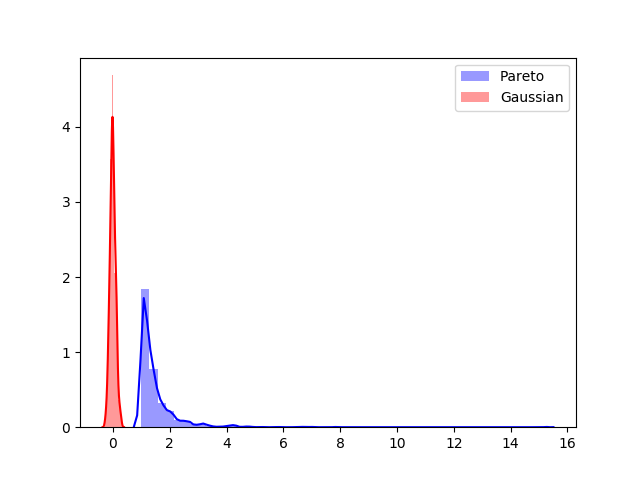
\includegraphics[width=0.8\textwidth]{figures/4_Xpg2.png}
	\caption{Pareto distribution and Gaussian contamination}
	\label{fig:4.01}
\end{figure}

The $\pmb{Y}_l^c$ denotes the Lognormal distribution contaminated by Gaussian noise, accordingly to depicted by to Figure \ref{fig:4.02}, where it is possible to observe the Lognormal legitimate distribution $\pmb{Y}_l$ and the addictive gaussian noise to simulate the anomalies.Z

\begin{figure}[!htb]
	\centering
	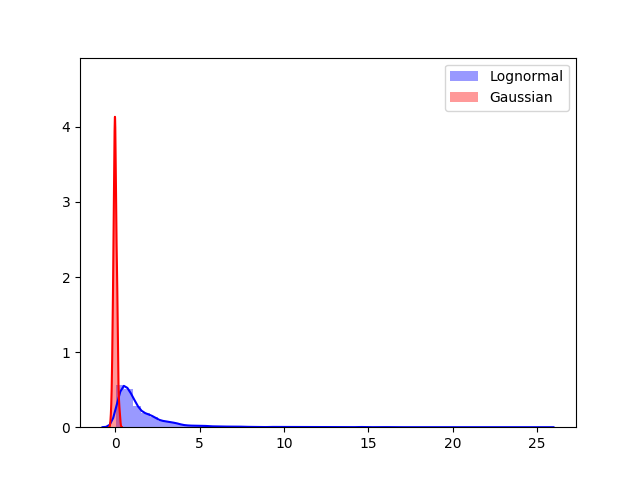
\includegraphics[width=0.8\textwidth]{figures/4_Xlogng2.png}=
	\caption{Lognormal distribution and Gaussian contamination}
	\label{fig:4.02}
\end{figure}

The figure \ref{fig:4.03} shows an example of the Gaussian distribution $\pmb{Y}_g$ of legitimate observations and the uniform distribution to simulate the addition of anomalies, composing the Gaussian distribution contaminated by uniform noise $\pmb{Y}_g^c$.

\begin{figure}[h!]
	\centering
	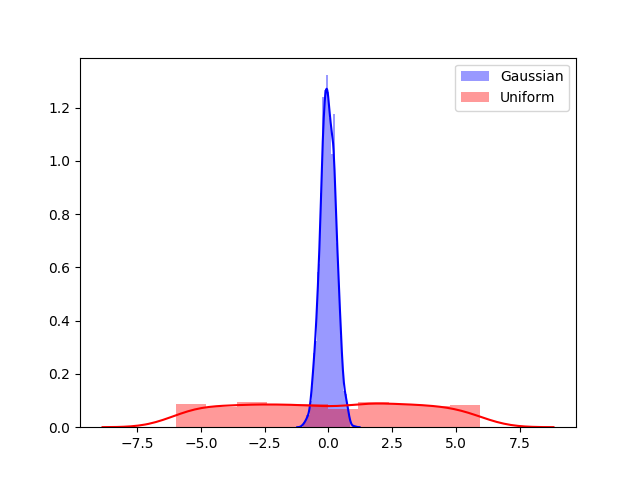
\includegraphics[width=0.8\textwidth]{figures/4_Xgu2.png}
	\caption{Example of Gaussian and Uniform Anomalies}
	\label{fig:4.03}
\end{figure}

Each contaminated data set is composed by a number of legitimate observations and contaminated samples. We evaluate contamination rates $c$ between 1\% and 50\%, to simulate the imbalanced data of anomaly detection problems during our experiments. This data set simulate a total of 2400 events for each scenario with contaminated Pareto, Lognormal or Gaussian distribution. Therefore, the number of legitimate observations is defined according to the contamination rate selected for each evaluation.


\subsection{The CTU-13 data set}
\label{sec:3_CTU-13}

The CTU-13 \cite{garcia2014empirical} is a data set of botnet traffic that was captured in the Czech Technical University, by means of a testbed and malware execution in a real network. The CTU-13 data set contains 13 scenarios with network flows of botnet malwares, that are: neris, rbot, virut, menti, sogou, nsys.ay and murlo. The botnet traffic is also classified as attack or command and control (C\&C), while the legitimate flows can also be classified as legitimate or background.

The types of C\&C and attack flows present in CTU-13 data set are:

\begin{itemize}
	\item \pmb{Attacks:} Click Fraud (CF), Port Scan (PS), Fast Flux (FF), SPAM and DDoS;
	\item \pmb{C\&C:} IRC, P2P and HTTP.
\end{itemize}

We refer to Garcia \cite{garcia2014identifying} and Garcia \emph{et al.} \cite{garcia2014empirical} for a detailed description of the performed attacks and C\&C flows, as well as for more information about the topology of the adopted testbed, rules for classifying legitimate flows, and an analysis of behaviors or patterns of the malware's traffic.

For all the scenarios, the authors of the CTU-13 data set convert the captured pcap files to NetFlows and release the processed flows. The data set provides ground-truth labels for flows as follows: flows from or to the infected machines are labeled as “botnet”; flows from or to well-known and controlled machines are labeled as “normal”; all other flows are labeled as “background.”

Table \ref{tab:4.01} presents an overview grouped by scenario, according to the column ID, and shows the malwares used for botnet attacks, the types of attacks or C\&C, the total number of flows, the number of malicious flows which includes flows of C\&C and attacks, and finally shows the number of legitimate flows.

\begin{table}[h!]
	\tiny
	\caption{CTU-13 data set description}
	\label{tab:4.01}
	\begin{tabular}{| l | l | l | r | r | r | r | r | r | r | r | }
		\hline \rowcolor{Gray} \begin{tabular}[x]{@{}l@{}}\textbf{ID}\end{tabular}	&\begin{tabular}[x]{@{}l@{}}\textbf{Bot}\end{tabular}	 &\begin{tabular}[x]{@{}l@{}}\textbf{Type}\end{tabular}	&\begin{tabular}[x]{@{}l@{}}\textbf{Total}\end{tabular} &\begin{tabular}[x]{@{}l@{}}\textbf{Malicious}\end{tabular} &\begin{tabular}[x]{@{}l@{}}\textbf{C\&C}\end{tabular} &\begin{tabular}[x]{@{}l@{}}\textbf{Attack}\end{tabular} &\begin{tabular}[x]{@{}l@{}}\textbf{Normal}\end{tabular}\\ \hline
			10 & neris &\makecell[l]{IRC,\\Spam,\\CF} & 2,824,636 & 40,961 (1.45\%) & 341 (0.01\%) & 40,620 (1.44\%) &30,387 (1.07\%)\\ \hline
			11 & neris &\makecell[l]{IRC,\\Spam,\\CF} & 1,808,122 & 20,941 (1.16\%) & 673 (0.04\%) & 20,268 (1.12\%) &9,120 (0.5\%)\\ \hline
			12 & rbot &\makecell[l]{IRC,\\PS} & 4,710,638 & 26,822 (0.57\%) & 63 (0.00\%) & 26,759 (0.57\%) &116,887 (2.48\%)\\ \hline
			15 & rbot &\makecell[l]{IRC,\\DDoS} & 1,121,076 & 2,580 (0.23\%) & 52 (0.00\%) & 2,528 (0.23\%) &25,268 (2.25\%)\\ \hline
			15-2 & virut &\makecell[l]{Spam,\\PS,\\HTTP} & 129,832 & 901 (0.69\%) & 24 (0.02\%) & 877 (0.68\%) &4,679 (3.6\%)\\ \hline
			16 & menti &PS & 558,919 & 4,630 (0.83\%) & 199 (0.04\%) & 4,431 (0.79\%) &7,494 (1.34\%)\\ \hline
			16-2 & sogou &HTTP & 114,077 & 63 (0.06\%) & 26 (0.02\%) & 37 (0.03\%) &1,677 (1.47\%)\\ \hline
			16-3 & murlo &PS & 2,954,230 & 6,127 (0.21\%) & 1,074 (0.04\%) & 5,053 (0.17\%) &72,822 (2.46\%)\\ \hline
			17 & neris &\makecell[l]{IRC,\\Spam,\\CF,\\PS} & 2,087,508 & 184,987 (8.86\%) & 2,973 (0.14\%) & 182,014 (8.72\%) &43,340 (1.57\%)\\ \hline
			18 & rbot &\makecell[l]{IRC,\\DDoS} & 1,309,791 & 106,352 (8.12\%) & 33 (0.00\%) & 106,319 (8.12\%) &15,847 (1.2\%)\\ \hline
			18-2 & rbot &\makecell[l]{IRC,\\DDoS} & 107,251 & 8,164 (7.61\%) & 2 (0.00\%) & 8,162 (7.61\%) &2,718 (2.53\%)\\ \hline
			19 & nsys.ay &P2P & 325,471 & 2,168 (0.67\%) & 25 (0.01\%) & 2,143 (0.66\%) &7,628 (2.35\%)\\ \hline
			15-3 & virut &\makecell[l]{Spam,\\PS,\\HTTP} & 1,925,149 & 40,003 (2.08\%) & 536 (0.03\%) & 39,467 (2.05\%) &31,939 (1.65)\\ \hline
	\end{tabular}
\end{table}

The full data set and scenarios can be denoted as $\pmb{X} = \{\pmb{X}_{10}, \pmb{X}_{11}, \ldots , \pmb{X}_{18-2},\\ \pmb{X}_{19}\}$, in accordance to IDs presented in Table \ref{tab:4.01}. In our experiment each contaminated scenario $\pmb{X}_i$ is split into $\pmb{X}_i^s$ containing 50\% of the legitimate data, and into $\pmb{X}_i^c$ that is composed by all anomalous flows and the necessary number of legitimate flows to have a testing data with the desired contamination rate.

The CTU-13 data set originally contains the following features for each flow: Start Time, End Time, Duration, Source IP Address, Source Port. Direction, Destination IP Address, Destination Port, State of TCP flags, Destination Type of Service, Source Type of Service, Total number of Packets, Total number of Bytes.

Our analysis of the available features leads to discard some features, considering that highly correlated features can bias or not improve the model, and that source or destination IP addresses can insert some false bias into learning models, since they can be changed by IP spoofing. Other risk related to adopt IP address for training models is the training model to learn that
one IP is legitimate and this IP be infected subsequently, which can result into false negative classifications.

We conducted and Exploratory Data Analysis (EDA) on the CTU-13 and observed that some features are skewed and present high overlapping between legitimate and anomalous flows, as can be seen in Figure \ref{fig:4.05} and Figure \ref{fig:4.06}, that present the distributions of TCP state of scenario 16 and the type of services from destination of scenario 10.

\begin{figure}[!htb]
	\centering
	\subfigure[State of scenario 16.]{%
		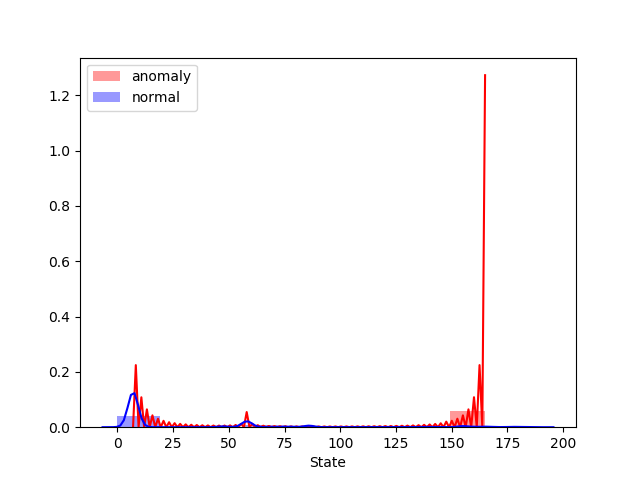
\includegraphics[width=0.47\textwidth]{figures/raw_distplot_capture20110816_State.png}
		\label{fig:4.05}
	}
	\subfigure[Destination Type of service of scenario 10.]{%
		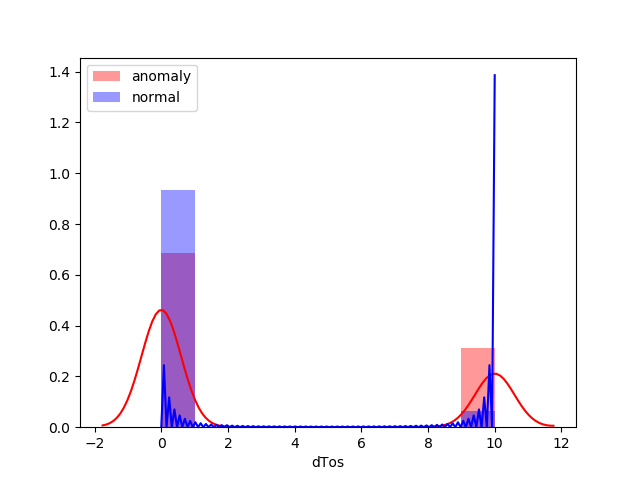
\includegraphics[width=0.47\textwidth]{figures/raw_distplot_capture20110810_dTos.png}
		\label{fig:4.06}
	}
	\caption[Skewness and Overlapping]{Example of skewness and overlapping}
	\label{fig:4.07}
\end{figure}

However, it is not possible to observe a pattern on distributions of all the features and scenarios of CTU-13, as depicted by Figures \ref{fig:4.08} and \ref{fig:4.09}, that show the distributions of TCP states of the scenario 10 and source ports of scenario 16, and highlight the distributions of legitimate and anomalous flows.

\begin{figure}[!htb]
	\centering
	\subfigure[State of scenario 10.]{%
		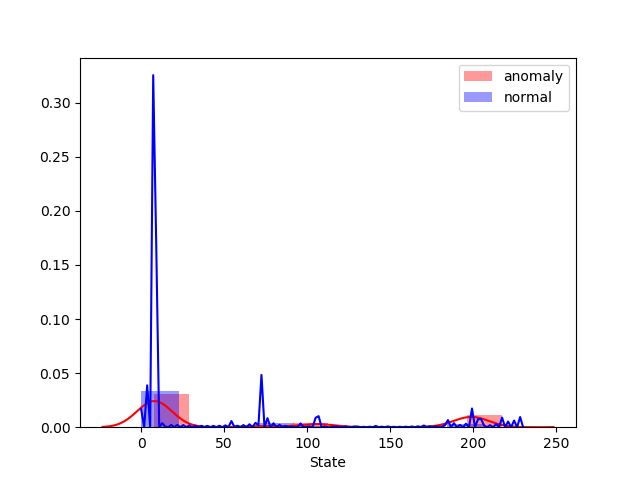
\includegraphics[width=0.47\textwidth]{figures/raw_distplot_capture20110810_State.png}
		\label{fig:4.08}
	}
	\subfigure[Source Port of scenario 16.]{%
		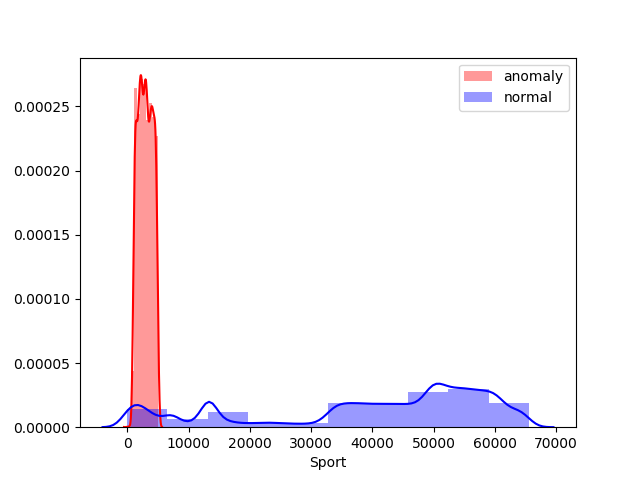
\includegraphics[width=0.47\textwidth]{figures/raw_distplot_capture20110816_Sport.png}
		\label{fig:4.09}
	}
	\caption[Skewness and Overlapping]{Skewness and Overlapping}
	\label{fig:4.10}
\end{figure}

Due to the number of available features and the class overlapping between legitimate and anomalous flows, we performed an correlation analysis and an empirical cross validation to identify the best set of features for network attack detection. Therefore, we adopt the following features: state, destination type of service, destination port, source port, total number of packets, total number of bytes and number of bytes from the source.

%%%%%%%%%%%%%%%%%%%%%%%%%%%%%%%%%%%%%%%%%%%%%%%%%%%%%%%%%%%%%%%%%%%%%%%%%%%%%%%%%%%%%%%%%%%%%%%%%%%%%%%%%%%%%%%%%%%%%%%%%%%%%%%%%%%%%%%%%%%%%%%%%%%%%%%%%%%%%%%%%%%%%%%%%%%%%%%%%%%%%%%%%%%%%%%%%%%%%%%%%%%%%%%%%%%%%%%%%%%%
\section{Moment Distances from Robust Subspace for Botnet Detection}
\label{sec:mdrs}


This section describes the proposed approach for network attack detection by means of a distance analysis between moments computed from a robust subspace and contaminated observations of network traffic. 

Robust subspace learning can be defined as the decomposition of a given data matrix $\pmb{X} \in \mathbb{R}^{M \times N}$, with rows representing observations and columns representing features. In this work we adopt a flow based analysis, where $\pmb{X}$ is modeled as a matrix of flows by features, and $\pmb{X}$ is decomposed into the sum of a low rank matrix $\pmb{L} \in \mathbb{R}^{M \times N}$, whose column subspace gives the robust principal components without outliers and noise, and a sparse matrix $\pmb{S} \in \mathbb{R}^{M \times N}$, with element-wise outliers or noise.

Even though robust subspace learning has been adopted for network anomaly detection by means of highlights from the matrix $\pmb{S}$, it was shown that $\pmb{S}$ can indicate noise and outliers that can not be classified as malicious \cite{vaswani2018robust, lerman2018overview}, resulting into false positive classifications and requiring complementary approaches to obtain precise network anomaly detection \cite{zhou2017anomaly}.

Therefore, for network anomaly detection, we propose to learn a robust subspace from the legitimate traffic $\pmb{X}^s$ for computing $\pmb{L}^s$ and $\pmb{S}^s$, followed by computing the robust moments, i.e. the mean $\pmb{\mu}$, skewness $\pmb{\epsilon}$ and kurtosis $\pmb{\kappa}$, to evaluate the distance $\pmb{d}$ between contaminated observations $\pmb{X}^c$ and robust moments. The largest distances are classified as anomalous and indicate network attacks, denoted as $\pmb{N}$ by the data model $\pmb{X} = \pmb{U} + \pmb{N}$, where $\pmb{U}$ denotes the legitimate network traffic.

RPCA is a well-known method to recover a low-rank matrix $\pmb{L}$ and sparse matrix $\pmb{S}$ from corrupted measurements modeled as $\pmb{X} = \pmb{L} + \pmb{S}$. This decomposition in low-rank and sparse matrices can be achieved by techniques such as Principal Component Pursuit method (PCP), and by optimization methods, such as the Augmented Lagrange Multiplier Method (ALM), Alternating Direction Method (ADM), Fast Alternating Minimization (FAM) or Iteratively Reweighted Least Squares (IRLS) \cite{candes2011robust,vaswani2018robust,lerman2018overview}.

According to Wright et al. \cite{wright2009robust}, under rather broad conditions, as long as the error matrix $\pmb{S}$ is sufficiently sparse, it is possible to recover a low-rank matrix by solving the following convex optimization problem:
\begin{equation}\label{eq:4.01}
	(\hat{\pmb{L}}, \hat{\pmb{S}})\leftarrow \min_{\pmb{L},\pmb{S}}\left \| \pmb{L} \right \|_{*} + \lambda \left \| \pmb{S} \right \|_{1}
\end{equation}
\begin{center} subject to: $\pmb{X} = \pmb{L} + \pmb{S}$ \end{center}
\begin{equation}\label{eq:4.02}
    \left \| \pmb{L} \right \|_{*} = \sum_{i} \sigma_{i}(\pmb{L})
\end{equation}
\begin{equation}\label{eq:4.03}
    \left \| \pmb{S} \right \|_{1} = \sum_{ij} \left | \pmb{S}_{ij} \right |
\end{equation}
where $\left\| \mathord{\cdot} \right\|_*$ denotes the nuclear norm of a matrix, $\lambda$ is a positive weighting parameter, which determines the sparsity of $\pmb{S}$, and $\left\| \mathord{\cdot} \right\|_1$ means the sum of the absolute values of matrix entries, and $\sigma$ denotes the singular values of a matrix. 

Before ALM, some methods were proposed to solve that convex optimization problem, such as Iterative Thresholding (IT) and Accelerated Proximal Gradient (APG). However, according to Zhouchen \emph{et al.} \cite{lin2010augmented}, both approaches have scalability problems and require a large number of iterations to converge. The Augmented Lagrange Multiplier (ALM) is proven to have a \emph{Q-linear} convergence speed and experimental results show that ALM is five times faster than APG, which in theory is sub-linear \cite{lin2010augmented}. Furthermore, ALM reaches more accurate results with less iterations.

The RPCA with ALM can be formulated as:
\begin{equation}\label{eq:4.04}
	l(\pmb{L}, \pmb{S}, \pmb{Y}) = \left\|\pmb{L}\right\|_* + \lambda\left\|\pmb{S}\right\|_1 + \langle \pmb{Y}, \pmb{X} - \pmb{L} - \pmb{S}  \rangle + \frac{\mu}{2}\left\|\pmb{X} - \pmb{L} - \pmb{S}\right\|_F^2,
\end{equation}
where $\pmb{Y}$ is the multiplier of the linear constraint and $\mu$ is the penalty parameter for the violation of the linear constraint \cite{yuan2009sparse}. 

Thus, an iterative scheme can be presented as:
\begin{equation}\label{eq:4.05}
	\left\{
		\begin{matrix} 
			(\pmb{L}_{k+1}, \pmb{S}_{k+1}) \in \argmin\limits_{\pmb{L,S} \in \mathbb{R}^{m \times n}} \{l(\pmb{L}, \pmb{S}, \pmb{Y}_{k})\}, \\ 
			\pmb{Y}_{k+1} = \pmb{Y}_{k} + \mu(\pmb{X} - \pmb{L}_{k} - \pmb{S}_{k}),
		\end{matrix}
	\right.
\end{equation}

We adopt RPCA with ADM, which, generally speaking, is a practical improvement of the classical ALM method for solving convex programming problem with linear constraints, by fully taking advantage of its high-level separable structure \cite{yuan2009sparse}. ADM minimizes $\pmb{L}$ and $\pmb{S}$ variables serially by solving the following problems to generate the new iterate:

\begin{equation}\label{eq:4.06}
	\left\{\begin{matrix}
	\pmb{L}_{k+1} \in \argmin\limits_{\pmb{L} \in \mathbb{R}^{m \times n}}\{l(\pmb{L}, \pmb{S}_{k}, \pmb{Y}_{k})\}\\ 
	\pmb{S}_{k+1} \in \argmin\limits_{\pmb{S} \in \mathbb{R}^{m \times n}}\{l(\pmb{L}_{k+1}, \pmb{S}, \pmb{Y}_{k})\}\\ 
	\pmb{Y}_{k+1} = \pmb{Y}_{k} + \mu(\pmb{X} - \pmb{L}_{k} - \pmb{S}_{k})
	\end{matrix}\right.
\end{equation}

Moments are a set of statistical parameters to measure a distribution. The arithmetic mean is the first general moment, the second is the variance, while skewness (asymmetry) is the third moment and kurtosis (tailedness) is the fourth moment \cite{reis2016audio}.

Let the mean $\pmb{\mu} \in \mathbb{R}^{1 \times N}$ be

\begin{equation}\label{eq:4.07}
	\pmb{\mu} = \displaystyle\frac{1}{M}\displaystyle\sum_{i = 1}^{M} \pmb{x}_i,
\end{equation}

where $M$ is the number of samples, and let the sample covariance matrix $\hat{\pmb{\Sigma}} \in \mathbb{R}^{N \times N}$ be

\begin{equation}\label{eq:4.08}
	\hat{\pmb{\Sigma}} = \displaystyle\frac{1}{N-1}\displaystyle\sum_{i = 1}^{N} (\pmb{x}_i - \pmb{\mu})(\pmb{x}_i - \pmb{\mu})^T,
\end{equation}

\begin{equation}\label{eq:4.08.1}
	\frac{1}{N-1} \sum_{i = 1}^{N} I_x1 (x_i - \mu ) _x2 (x_i - \mu) 
\end{equation}



According to Zwillinger and Kokoska \cite{zwillinger1999crc}, the general expression for the $p$-th moment $\pmb{m}_p \in \mathbb{R}^{1 \times N}$ about the mean $\pmb{\mu}$ is given by
\begin{equation}\label{eq:4.09}
	\pmb{m}_p = \displaystyle\frac{1}{M}\displaystyle\sum_{i = 1}^{M}(\pmb{x}_i - \pmb{\mu})^p.
\end{equation}

Therefore, Zwillinger and Kokoska \cite{zwillinger1999crc} present that the skewness $\pmb{\epsilon} \in \mathbb{R}^{1 \times N}$ about the mean $\pmb{\mu}$ is calculated by
\begin{equation}\label{eq:4.10}
	\pmb{\epsilon} = \frac{\pmb{m}_3}{\pmb{m}_2^{\frac{3}{2}}},
\end{equation}

and the kurtosis $\pmb{\kappa} \in \mathbb{R}^{1 \times N}$ is given as
\begin{equation}\label{eq:4.11}
	\pmb{\kappa} = \frac{\pmb{m}_4}{\pmb{m}_2^2}.
\end{equation}

We propose to compute the mean $\pmb{\mu}$, the skewness $\pmb{\epsilon}$, the kurtosis $\pmb{\kappa}$ and the covariance matrix $\hat{\pmb{\Sigma}}$ from the robust subspace $\pmb{L}^s$, after to minimize the (\ref{eq:4.06}) for $\pmb{X}^s$. We also propose to compute the Mahalanobis Distance (MD) for detecting anomalies between contaminated observations and the moments calculated from a robust subspace computed by RPCA. 

The classical Mahalanobis Distance is defined as		
\begin{equation}\label{eq:4.12}
	\pmb{d}(\pmb{x}, \pmb{\mu}, \hat{\pmb{\Sigma}}) = \sqrt{(\pmb{x} - \pmb{\mu}) \hat{\pmb{\Sigma}}^{-1}(\pmb{x} - \pmb{\mu})^T},
\end{equation}
where $\pmb{x}$ is a vector of a new observations, $\pmb{\mu}$ is the mean vector of known observations, also referred as location, and $\hat{\pmb{\Sigma}}$ is the covariance matrix of known observations, also referred as scatter. The classical MD usually relies on robust mean and robust covariance matrix for outlier detection, which are commonly computed by MCD \cite{rousseeuw1984mcd, rousseeuw1999fastmcd}. Here we propose to compute the Robust-Mean Distance $\pmb{d}(\pmb{x}, \pmb{\mu}, \hat{\pmb{\Sigma}})$ according to (\ref{eq:4.12}), but adopting the mean $\pmb{\mu}$ and covariance matrix $\hat{\pmb{\Sigma}}$ calculated from a robust subspace $\pmb{L}^s$ learned by RPCA.

We also propose to extend (\ref{eq:4.12}) to implement the Robust-Skewness Distance $\pmb{d}(\pmb{x}, \pmb{\epsilon}, \hat{\pmb{\Sigma}})$, as follows:

\begin{equation}\label{eq:4.13}
	\pmb{d}(\pmb{x}, \pmb{\epsilon}, \hat{\pmb{\Sigma}}) = \sqrt{(\pmb{x} - \pmb{\epsilon}) \hat{\pmb{\Sigma}}^{-1}(\pmb{x} - \pmb{\epsilon})^T}.
\end{equation}

Finally, we propose to extend (\ref{eq:4.12}) to implement the Robust-Kurtosis Distance $\pmb{d}(\pmb{x}, \pmb{\kappa}, \hat{\pmb{\Sigma}})$, as follows:

\begin{equation}\label{eq:4.14}
	\pmb{d}(\pmb{x}, \pmb{\kappa}, \hat{\pmb{\Sigma}}) = \sqrt{(\pmb{x} - \pmb{\kappa}) \hat{\pmb{\Sigma}}^{-1}(\pmb{x} - \pmb{\kappa})^T}.
\end{equation}

The distances $\pmb{d}(\pmb{x}, \pmb{\mu}, \hat{\pmb{\Sigma}})$, $\pmb{d}(\pmb{x}, \pmb{\epsilon}, \hat{\pmb{\Sigma}})$ and $\pmb{d}(\pmb{x}, \pmb{\kappa}, \hat{\pmb{\Sigma}})$ shall be computed and evaluated separately and independently, for network attack detection based on robust mean, robust skewness and robust kurtosis, respectively. 

Therefore, the robust subspace $\pmb{L}^s$ learned from legitimate data $\pmb{X}^s$ followed by the Robust-Mean Distance $\pmb{d}(\pmb{x}, \pmb{\mu}, \hat{\pmb{\Sigma}})$ is called as Mean Distance of Robust Principal Component Analysis (md-RPCA), or is called Skewness Distance of Robust Principal Component Analysis (sd-RPCA) when followed by Robust-Skewness Distance, given by $\pmb{d}(\pmb{x}, \pmb{\epsilon}, \hat{\pmb{\Sigma}})$, or Kurtosis Distance of Robust Principal Component Analysis (kd-RPCA) when followed by Robust-Kurtosis Distance, given by $\pmb{d}(\pmb{x}, \pmb{\kappa}, \hat{\pmb{\Sigma}})$.

The contamination rate, denoted by $c$, is a parameter traditionally adopted by well established outlier detection algorithms \cite{zhao2019pyod}, and refers to the percentage rate of observations that are known as anomalous. The contamination rate can be well-known for some areas, or can be computed by cross-validation \cite{arlot2010survey} or can be assumed according to previous observations. In our proposal, the contamination defines the number of the largest distances $\pmb{d}(\pmb{x}, \pmb{\mu}, \hat{\pmb{\Sigma}})$, $\pmb{d}(\pmb{x}, \pmb{\epsilon}, \hat{\pmb{\Sigma}})$ or $\pmb{d}(\pmb{x}, \pmb{\kappa}, \hat{\pmb{\Sigma}})$ that shall be classified as anomalous. The observations classified as legitimate and anomalous, according to the contamination $c$, are denoted by the vector $\hat{\pmb{t}}$, with values of 1 for observations classified as anomalous and 0 to denote legitimate observations.

The Algorithm \ref{alg:4.01} describes all possible steps of m-RPCA and the approaches md-RPCA, sd-RPCA and kd-RPCA, for the semi-supervised learning approach. The unsupervised approach adopts the same steps, but adopting the contaminated data for robust subspace learning, and requiring new robust subspace learning for testing anomaly detection on new set of observations.

\begin{algorithm}
	\label{alg:4.01}
	\SetAlgoLined
	\KwResult{$\hat{\pmb{t}}_{\mu}$, $\hat{\pmb{t}}_{\epsilon}$, $\hat{\pmb{t}}_{\kappa}$}
	Given $\pmb{X}$ split into $\pmb{X}^s$ and $\pmb{X}^c$\;
	\While{\rm not $\min_{L,S}\left \| \pmb{L} \right \|_{*} + \lambda \left \| \pmb{S} \right \|_{1}$ \rm from $\pmb{X}^s$}{
		$\pmb{L}_{k+1} \in \argmin\limits_{\pmb{L} \in \mathbb{R}^{m \times n}}\{l(\pmb{L}, \pmb{S}_{k}, \pmb{Y}_{k})\}$\;
		$\pmb{S}_{k+1} \in \argmin\limits_{\pmb{S} \in \mathbb{R}^{m \times n}}\{l(\pmb{L}_{k+1}, \pmb{S}, \pmb{Y}_{k})\}$\;
		$\pmb{Y}_{k+1} = \pmb{Y}_{k} + \mu(\pmb{X} - \pmb{L}_{k} - \pmb{S}_{k})$\;
	}
	$\pmb{\mu} = \displaystyle\frac{1}{M}\displaystyle\sum_{i = 1}^{M} \pmb{x}_i$, from $\pmb{L}$\;
	$\hat{\pmb{\Sigma}} = \displaystyle\frac{1}{N-1}\displaystyle\sum_{i = 1}^{N} (\pmb{x}_i - \pmb{\mu})(\pmb{x}_i - \pmb{\mu})^T$, \rm from $\pmb{L}$\;
	$\pmb{\epsilon} = \frac{\pmb{m}_3}{\pmb{m}_2^{\frac{3}{2}}}$, \rm from $\pmb{L}$\;
	$\pmb{\kappa} = \frac{\pmb{m}_4}{\pmb{m}_2^2}$, \rm from $\pmb{L}$\;
	$\pmb{d}(\pmb{x}, \pmb{\mu}, \hat{\pmb{\Sigma}}) = \sqrt{(\pmb{x} - \pmb{\mu}) \hat{\pmb{\Sigma}}^{-1}(\pmb{x} - \pmb{\mu})^T}$, \rm from $\pmb{X}^c$\;
	$\pmb{d}(\pmb{x}, \pmb{\epsilon}, \hat{\pmb{\Sigma}}) = \sqrt{(\pmb{x} - \pmb{\epsilon}) \hat{\pmb{\Sigma}}^{-1}(\pmb{x} - \pmb{\epsilon})^T}$, \rm from $\pmb{X}^c$\;
	$\pmb{d}(\pmb{x}, \pmb{\kappa}, \hat{\pmb{\Sigma}}) = \sqrt{(\pmb{x} - \pmb{\kappa}) \hat{\pmb{\Sigma}}^{-1}(\pmb{x} - \pmb{\kappa})^T}$, \rm from $\pmb{X}^c$\;
	$\hat{\pmb{t}}_{\mu} = [\pmb{d}(\pmb{x}, \pmb{\mu}, \hat{\pmb{\Sigma}})]^c$\;
	$\hat{\pmb{t}}_{\epsilon} = [\pmb{d}(\pmb{x}, \pmb{\epsilon}, \hat{\pmb{\Sigma}})]^c$\;
	$\hat{\pmb{t}}_{\kappa} = [\pmb{d}(\pmb{x}, \pmb{\kappa}, \hat{\pmb{\Sigma}})]^c$\;
	\caption{Moment Distances from Robust Subspace}
\end{algorithm}

The steps between 1 and 10 of the Algorithm \ref{alg:4.01} are the training from legitimate data $\pmb{X}^s$, which are common steps shared by md-RPCA, sd-RPCA and kd-RPCA. The steps between 11 and 16 aim the anomaly detection from new contaminated observations, by means of Mahalanobis Distance of robust moments. Note that the steps 11 and 14 refer to the steps of md-RPCA for anomaly detection, while the steps 12 and 15 refer to the sd-RPCA, and the steps 13 and 16 refer to the steps of kd-RPCA. It is important to highlight that the anomaly detection from new observations does not require new robust subspace learning when adopting the semi-supervised approach, which only requires to compute a moment-based distance to classify the $c$ largest distances as anomalous or legitimate.

The m-RPCA can also be adopted as unsupervised algorithm if the lines 1 and 2 of the Algorithm \ref{alg:4.01} are changed to substitute $\pmb{X}^s$ by $\pmb{X}^c$. Hence, the robust subspace is learned from contaminated data and used for comparing the distance between moments from robust estimate and contaminated observations. It is important to note that this unsupervised approach requires the computational cost of computing new subspace learning for any new set of observations.


%%%%%%%%%%%%%%%%%%%%%%%%%%%%%%%%%%%%%%%%%%%%%%%%%%%%%%%%%%%%%%%%%%%%%%%%%%%%%%%%%%%%%%%%%%%%%%%%%%%%%%%%%%%%%%%%%%%%%%%%%%%%%%%%%%%%%%%%%%%%%%%%%%%%%%%%%%%%%%%%%%%%%%%%%%%%%%%%%%%%%%%%%%%%%%%%%%%%%%%%%%%%%%%%%%%%%%%%%%%%
\section{Experiments and Results}
\label{sec:experimentalresults}


This section presents the performed experiments on simulated and real data set for anomaly detection. First, in Section \ref{sec:3_metric} we present the adopted metric to evaluate imbalanced data in the context of anomaly detection. In Section \ref{sec:3_SimulatedScenario} we describe the experiment for anomaly detection on simulated skewed and heavy-tailed data set, and we present in Section \ref{sec:3_CTU-13} the experiment for network anomaly detection on CTU-13 data set.

\subsection{The metric}
\label{sec:3_metric}

In anomalous detection problems, where anomalies are rare events, if one classify all observations as legitimate and apply an accuracy evaluation, one would have high accuracy but poor true-positive detection. Due to the importance given by the $F_1$ (also referred as F-score or F-measure) to true-positive detection in scenarios such as the network attack detection, it is the preferable measure for imbalanced data \cite{powers2011evaluation,moustafa2019holistic}. Therefore, $F_1$ is the metric used for validation of our experiments.

The $F_1$ is the harmonic mean of precision and recall, where $p_{\rm p}$ denotes the precision and recall is denoted as $r_{\rm c}$. The $F_1$ is given by
\begin{equation}\label{eq:4.15}
	F_1 = 2 \cdot \frac{p_{\rm r} \cdot r_{\rm c}}{p_{\rm r} + r_{\rm c}}.
\end{equation}

Precision can be seen as a measure of exactness or accuracy, that relies on true positive and false positive measures, denoted by $t_{\rm p}$ and $f_{\rm p}$, respectively. The precision is defined by 
\begin{equation}\label{eq:4.16}
	p_r = \frac{t_{\rm p}}{t_{\rm p} + f_{\rm p}}.
\end{equation}

Recall is a measure of completeness, to calculate proportion of actual positives was identified correctly, by means of the true positive and false negative measures, denoted by $t_{\rm p}$ and $f_{\rm n}$. The recall is defined by 
\begin{equation}\label{eq:4.17}
	r_c = \frac{t_{\rm p}}{t_{\rm p} + f_{\rm n}}.
\end{equation}

This experimental evaluation compares our proposal to widely adopted algorithms for anomaly detection that also rely on contamination rate for anomaly detection, which are: A PCA approach based on the sum of weighted projected distances to the eigenvector hyperplanes \cite{shyu2003novel}; MCD \cite{rousseeuw1984mcd,rousseeuw1999fastmcd}; One-Class Support Vector Machines \cite{scholkopf2001estimating}; Local Outlier Factor (LOF) \cite{breunig2000lof}; k-Nearest Neighbors \cite{angiulli2002fast}; and Isolation Forest \cite{liu2008isolation}.

We also compare the results of our proposals to ROBPCA-AO for anomaly detection on simulated and CTU-13 data set, considering that ROBPCA-AO also relies on robust estimates with adjusted outlyingness based on robust skewness \cite{hubert2009robustskewed}.

\subsection{Simulated Experiment}
\label{sec:3_SimulatedScenario}

Anomaly detection algorithms usually rely on supervised or unsupervised methods, where the former requires labeled legitimate and anomalous data for training anomaly detection models, while the latter does not require labeled data or training. Semi-supervised algorithms are an alternative for the anomaly detection problem, considering that this method only relies on legitimate data for training and that non-malicious data can be obtained from historical information and from rule-based approaches. 

We propose semi-supervised and unsupervised approaches for m-RPCA, where the former relies on legitimate data $\pmb{X}^s$ for training and on contamination rate $c$ for anomaly detection, while the latter relies only on contaminated data $\pmb{X}^c$ for robust subspace learning and relies on contamination rate $c$ to select the largest distances. We assume that $c$ is well-known or can be estimated for real world problems of anomaly detection, in accordance to the assumption adopted by the well established algorithms \cite{zhao2019pyod} selected for comparison, that also rely on contamination rate $\pmb{X}^c$.

The availability of labeled data is a challenging concern in real world problems of anomalous detection, where anomalies are rare or even unknown events. Considering that RPCA has already been adopted to isolate outliers from training data \cite{zhou2017anomaly}, we also propose to evaluate the m-RPCA for a contaminated semi-supervised approach based on training from contaminated data, to evaluate the impact that contaminated data for robust subspace learning can cause in the anomaly detection results.

Therefore, we propose to evaluate the following approaches for m-RPCA: semi-supervised, contaminated semi-supervised, and unsupervised.

For the semi-supervised approach we propose to learn the robust subspace and compute the moments from the legitimate data $\pmb{Y}_g$, $\pmb{Y}_p$ and $\pmb{Y}_l$ with Gaussian, Pareto and Lognormal distributions, respectively, and test the anomaly detection for contaminated data $\pmb{Y}_g^c$, $\pmb{Y}_p^c$ and $\pmb{Y}_l^c$.

For the Contaminated Semi-supervised approach we evaluate the robustness of the m-RPCA approaches for learning from contaminated training data, to analyze if m-RPCA can be an alternative for the lack of known legitimate data. Therefore we propose to train the model from a contaminated legitimate data $\pmb{Y}_g^{c'}$, $\pmb{Y}_p^{c'}$ and $\pmb{Y}_l^{c'}$, with the same contamination rate of the testing data, but without data repetition between training and testing, taking into account that we shall consider a different contaminated data but adopt the same contamination rate for training and testing.

We finally evaluate the unsupervised approach, that relies on the test data $\pmb{Y}_g^c$, $\pmb{Y}_p^c$ and $\pmb{Y}_l^c$ for robust subspace learning, and then classify the results according to the distance between the contaminated data $\pmb{Y}_g^c$, $\pmb{Y}_p^c$ and $\pmb{Y}_l^c$, and the moments computed from the learned robust subspace.

\subsection{Experiment for CTU-13}
\label{sec:3_CTU13Scenario}

In contrast to Garcia \emph{et al.} \cite{garcia2014empirical}, we propose to evaluate each scenario of the CTU-13 data set individually, in a semi-supervised approach that does not rely on training data with labeled anomalies, to evaluate our proposed approaches to all botnet malwares of the CTU-13 data set. 

In our experiment setup each contaminated scenario $\pmb{X}_i$ of CTU-13 is split into $\pmb{X}_i^s$, containing 50\% of the legitimate data, and into test data $\pmb{X}_i^c$ containing 33\% of legitimate and 67\% of anomalous data. We adopt a contamination rate $c$ of 33\% for  experimenting anomaly detection for the CTU-13 data set, considering that this contamination rate presented good results on the simulated experiment for our proposals and for some selected algorithms.

This experiment consider only the semi-supervised approach due to results of simulated experiments on simulated data set presented in Subsection \ref{sec:3_simulated_result}, that shows better results for the semi-supervised approach and highlight that the this approach can obtain good results even when trained with contaminated data set.

\subsection{Results of Simulated Experiment}
\label{sec:3_simulated_result}

We adopt prefixes to denote the evaluated approaches for md-RPCA, sd-RPCA and kd-RPCA, which are ss\_ to denote semi-supervised, css\_ to denote contaminated semi-supervised and u\_ for unsupervised.

Initially, we evaluated the $F_1$ of the selected algorithms and m-RPCA approaches for anomaly detection on Gaussian distributed legitimate data contaminated by uniform distributed anomalies. The Figure \ref{fig:4.10} shows the $F_1$ over the contamination rate between 1\% and 50\% for m-RPCA approaches and Isolation Forest (IF) \cite{liu2008isolation}, k-Nearest Neighbors (KNN) \cite{angiulli2002fast}, Local Outlier Factor (LOF) \cite{breunig2000lof}, Minimum Covariance Deteminant (MCD) \cite{rousseeuw1999fastmcd}, One-Class Support Vector Machines (OCSVM) \cite{scholkopf2001estimating}, PCA \cite{shyu2003novel} and ROBPCA-AO \cite{hubert2009robustskewed}.

\begin{figure}[h!]
	\centering
	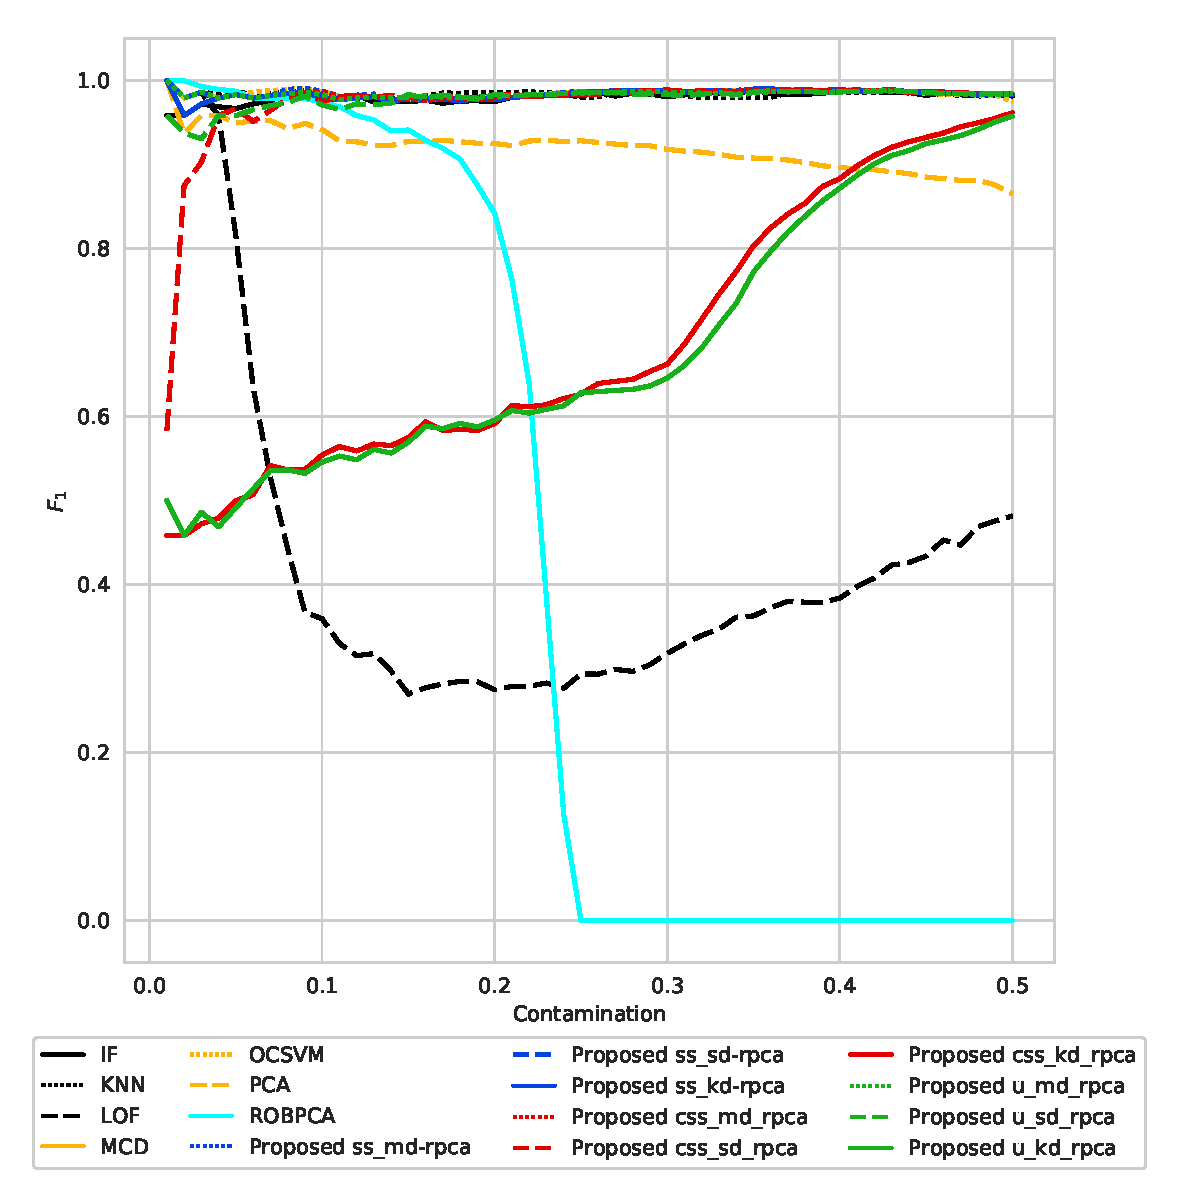
\includegraphics[width=10cm]{figures/gaussian_f1_contamination.eps}
	\caption{Anomaly detection on Gaussian distributed with uniform anomalies}
	\label{fig:4.10}
\end{figure}

It is possible to observe in Figure \ref{fig:4.10} that LOF, PCA, css\_kd-RPCA and u\_kd-RPCA presented lower performance than the remain algorithms, that obtain results higher than 0.95 in average, for anomaly detection on Gaussian distributed data. The exception is the ROBPCA-AO, that presented high score for lower contamination but decreased with the contamination increasing. 

Note that the css\_kd-RPCA and u\_kd-RPCA are the contaminated semi-supervised and unsupervised versions of kd-RPCA, that obtain worse results than the semi-supervised approach of kd-RPCA, for anomaly detection on Gaussian distributed data contaminated by uniform anomalies. However, the unsupervised versions of md-RPCA and sd-RPCA presented similar results to widely adopted unsupervised algorithms for outlier detection. The results also show that the semi-supervised approach of md-RPCA, sd-RPCA and kd-RPCA obtain high anomaly detection rate on Gaussian distributed data and presented similar results to the unsupervised algorithms IF, KNN, MCD and OCSVM. 

The Figure \ref{fig:4.11} and \ref{fig:4.12} show the results for anomaly detection on skewed and heavy tailed distributions, presenting results for anomaly detection on Pareto and Lognormal distributions, respectively.

\begin{figure}[h!]
	\centering
	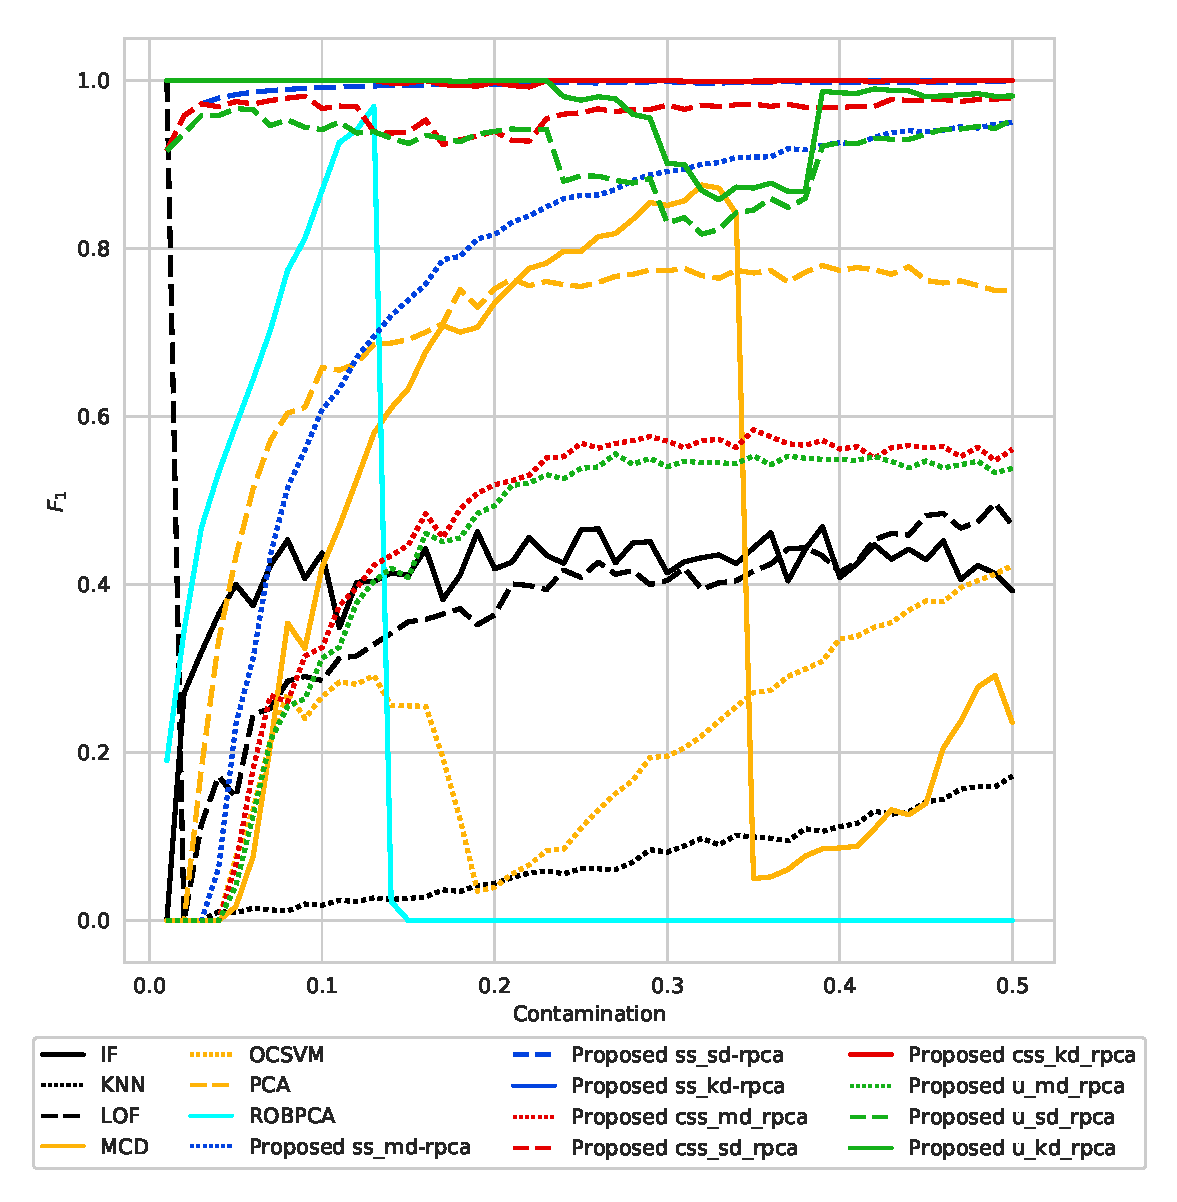
\includegraphics[width=10cm]{figures/pareto_f1_contamination.eps}
	\caption{Anomaly detection on Pareto distributed with Gaussian anomalies}
	\label{fig:4.11}
\end{figure}

The Figure \ref{fig:4.11} depics the results for anomaly detection on Pareto legitimate data with Gaussian anomalies, and shows that IF, KNN, LOF, OCSVM, css\_md-RPCA and u\_md-RPCA performed worse than the remain algorithms for the evaluated contamination, with results lower than 0.6 even with higher contamination. Note that the approaches of m-RPCA with lower scores are css\_md-RPCA and u\_md-RPCA, which are mean-based approaches. However, the ss\_md-RPCA is the mean-based approach that presented lower results for lower contamination but achieved more than 0.8 with contamination near of 0.2 or higher, and achieved results better than MCD and PCA.

Figure \ref{fig:4.11} shows that ROBPCA-AO presented high $F_1$ score for low contamination rates, presenting better results than ss\_md-RPCA, MCD and PCA for anomaly detection on Pareto distributed data, initially. However, the results of ROBPCA-AO decrease drastically with the contamination increasing. It is also possible to observe in Figure \ref{fig:4.11} that all approaches based on kd-RPCA initially achieved the best results for anomaly detection on Pareto distributed data, but the results for the unsupervised variate with contamination near of 0.2 or higher, while the ss\_kd-RPCA presents stable results, near of 1.0 $F_1$, for all evaluated contamination rates.

All approaches based on sd-RPCA obtained a $F_1$ score higher than 0.8 for anomaly detection on Pareto distributed data, however the unsupervised and contaminated semi-supervised presented high variation of $F_1$ and lower results in comparison to the semi-supervised sd-RPCA. The contaminated semi-supervised approaches of sd-RPCA and kd-RPCA presented higher results than 0.8 and similar to the semi-supervised and unsupervised approaches of sd-RPCA and kd-RPCA. These results highlight the resilience of the robust subspace learning even for contaminated training data.

The unsupervised approaches of sd-RPCA and kd-RPCA presented more than 0.8 for all contamination rate, showing better results than the widely adopted unsupervised algorithms for outlier detection. However, u\_kd-RPCA and u\_sd-RPCA presented lower results than ss\_kd-RPCA and ss\_sd-RPCA. 

Therefore, the semi-supervised approaches of m-RPCA overcome other approaches of m-RPCA and overcome the selected algorithms for anomaly detection on Pareto distributed data with Gaussian anomalies. Finally, it is possible to highlight the semi-supervised kd-RPCA, which obtained stable results near of 1.0 $F_1$ for all evaluated contamination.

The results for anomaly detection on Lognormal legitimate data with Gaussian anomalies is depicted by Figure \ref{fig:4.12}, and show that IF, KNN, LOF, MCD, OCSVM, css\_md-RPCA, u\_md-RPCA and ROBPCA-AO perform worse than the remain evaluated algorithms, with results lower than 0.6, even with higher contamination.

\begin{figure}[h!]
	\centering
	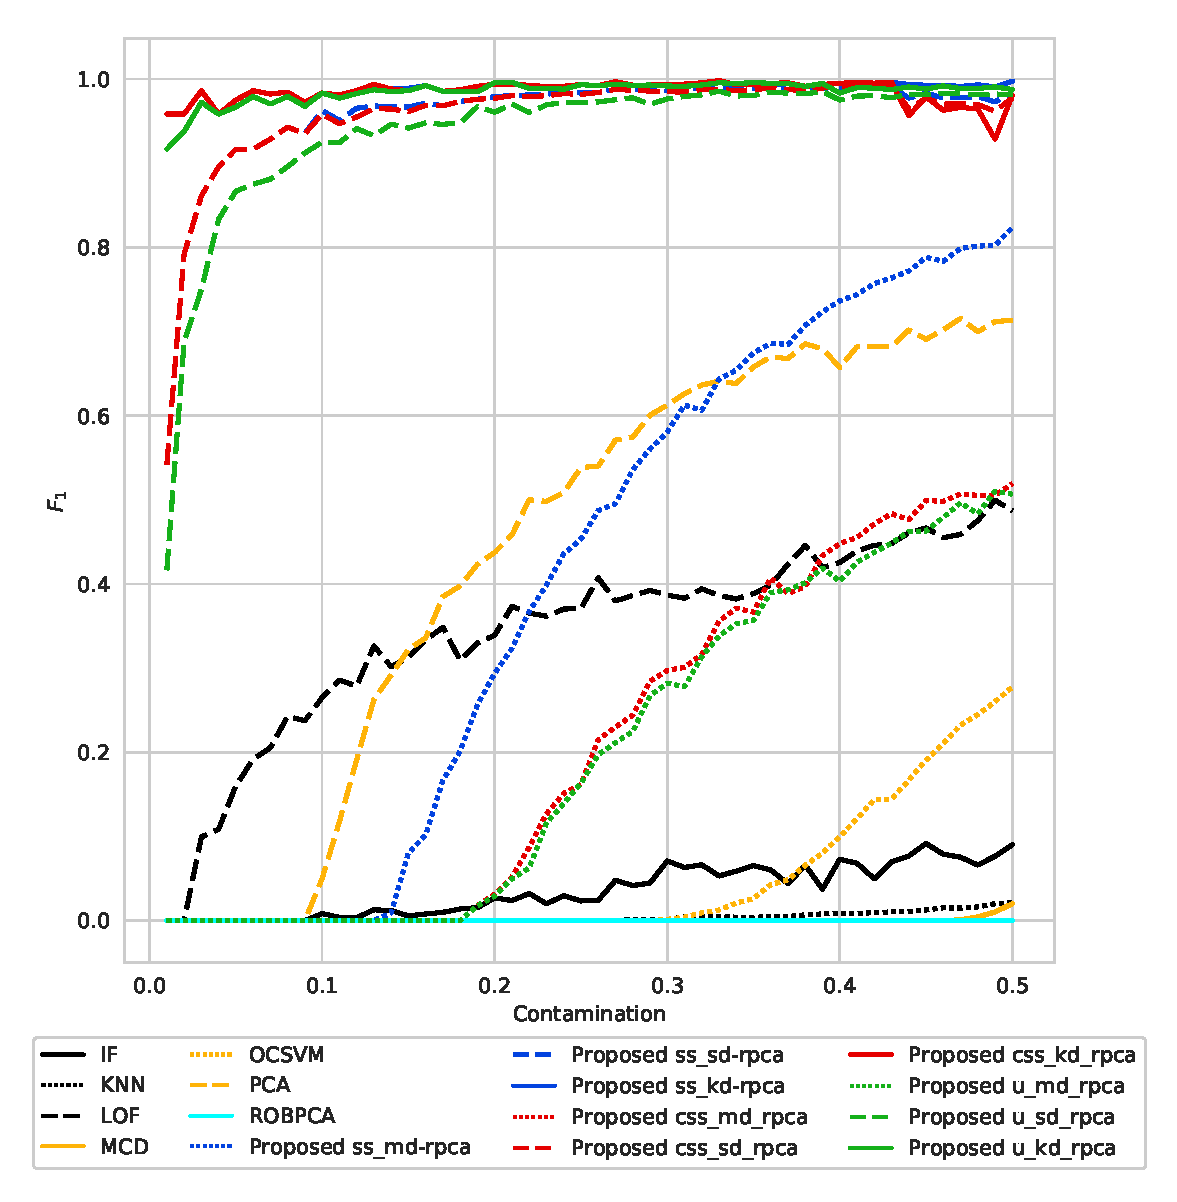
\includegraphics[width=10cm]{figures/lognormal_f1_contamination.eps}
	\caption{Anomaly detection on Lognormal distributed with Gaussian anomalies}
	\label{fig:4.12}
\end{figure}

The ss\_md-RPCA and PCA algorithms perform similar for anomaly detection on Lognormal distributed data, with worse detection rate for lower contamination and better performance with contamination higher than 0.4. However, the results of ss\_md-RPCA and PCA are lower than all approaches of sd-RPCA and kd-RPCA. 

It is important to note that all mean-based approaches of m-RPCA presented lower results for anomaly detection on Lognormal data, in comparison to approaches based on skewness (sd-RPCA) and kurtosis (kd-RPCA), that achieved the best anomaly detection rates. However, the approaches of md-RPCA presented better results than IF, KNN, MCD, OCSVM and ROBPCA-AO.

The approaches based on kd-RPCA presented higher detection rate for all contamination, with scores near of 1.0. The semi-supervised and contaminated semi-supervised approaches for sd-RPCA performed similarly, but the unsupervised approach of sd-RPCA presented lower anomaly detection on Lognormal distributed data, for lower contamination.

It is possible to note that the contaminated semi-supervised approaches of kd-RPCA and sd-RPCA performed similar to the semi-supervised approach of the same algorithms. These results highlight the resilience of the robust subspace learning, even from contaminated training data.

Finally, it is possible to observe that the semi-supervised approaches of m-RPCA overcome other approaches of m-RPCA and all the selected algorithms for anomaly detection on Lognormal distributed data with Gaussian anomalies. 

Following we present the Tables \ref{tab:4.02}, \ref{tab:4.03} and \ref{tab:4.04} to show the results of the selected algorithms and m-RPCA for anomaly detection on Gaussian, Pareto and Lognormal distributions, with 10\%, 25\% and 33\% of contamination rate. The columns present the $F_1$ score for each scenario, sorted by the best $F_1$.

\begin{table}[h!]
    \centering
	\scriptsize
	\caption{Results for Simulated data set with 33\% of contamination}
	\label{tab:4.02}
	\begin{tabular}{| l | l | l | l |}
		\hline \rowcolor{Gray} \begin{tabular}[x]{@{}c@{}}\textbf{Algorithm}\end{tabular}	&\begin{tabular}[x]{@{}c@{}}\textbf{Gaussian} \\+\textbf{Uniform} \end{tabular}	&\begin{tabular}[x]{@{}c@{}}\textbf{Pareto}+\\\textbf{Gaussian} \end{tabular}	 &\begin{tabular}[x]{@{}c@{}}\textbf{Lognormal} \\+\textbf{Gaussian} \end{tabular}\\ \hline
        	Proposed Semi-Supervised sd-RPCA	&0.98	&0.99	&0.97	\\ \hline
        	Proposed Semi-Supervised kd-RPCA	&0.97	&0.99	&0.98	\\ \hline
        	Proposed Contaminated Semi-Supervised sd-RPCA	&0.98	&0.94	&0.96	\\ \hline
        	Proposed Unsupervised sd-RPCA	&0.98	&0.82	&0.93	\\ \hline
        	Proposed Contaminated Semi-Supervised kd-RPCA	&0.76	&0.99	&0.98	\\ \hline
        	Proposed Unsupervised kd-RPCA	&0.74	&0.86	&0.99	\\ \hline
        	Proposed Semi-Supervised md-RPCA	&0.98	&0.90	&0.66	\\ \hline
        	PCA \cite{shyu2003novel}	&0.87	&0.76	&0.62	\\ \hline
        	Proposed Contaminated Semi-Supervised md-RPCA	&0.98	&0.55	&0.35	\\ \hline
        	Proposed Unsupervised md-RPCA	&0.98	&0.54	&0.31	\\ \hline
        	Isolation Forest \cite{liu2008isolation}	&0.98	&0.44	&0.05	\\ \hline
        	One-class SVM \cite{scholkopf2001estimating}	&0.98	&0.24	&0.00	\\ \hline
        	KNN \cite{angiulli2002fast}	&0.98	&0.08	&0.00	\\ \hline
        	MCD \cite{rousseeuw1999fastmcd}	&0.98	&0.02	&0.00	\\ \hline
        	LOF \cite{breunig2000lof}	&0.35	&0.40	&0.36	\\ \hline
        	ROBPCA-AO \cite{hubert2009robustskewed}		&0.00	&0.00	&0.00	\\ \hline
	\end{tabular}
\end{table}

The results for 33\% of contamination show high scores of anomaly detection for Gaussian data with uniform anomalies for the evaluated algorithms, with exception of LOF and ROBPCA-AO. The semi-supervised approaches of m-RPCA presented the highest results for anomaly detection on Pareto data with Gaussian anomalies, and for anomaly detection on Lognormal data with Gaussian anomalies, as well as for Gaussian data with uniform anomalies.

\begin{table}[h!]
    \centering
	\scriptsize
	\caption{Results for Simulated data set with 25\% of contamination}
	\label{tab:4.03}
	\begin{tabular}{| l | l | l | l |}
		\hline \rowcolor{Gray} \begin{tabular}[x]{@{}c@{}}\textbf{Algorithm}\end{tabular}	&\begin{tabular}[x]{@{}c@{}}\textbf{Gaussian} \\+\textbf{Uniform} \end{tabular}	&\begin{tabular}[x]{@{}c@{}}\textbf{Pareto}+\\\textbf{Gaussian} \end{tabular}	 &\begin{tabular}[x]{@{}c@{}}\textbf{Lognormal} \\+\textbf{Gaussian} \end{tabular}\\ \hline
            Proposed Semi-Supervised kd-RPCA    &0.96  &1.00  &0.98  \\ \hline
            Proposed Semi-Supervised sd-RPCA    &0.97  &0.99  &0.96  \\ \hline
            Proposed Contaminated Semi-Supervised sd-RPCA   &0.97  &0.91  &0.95  \\ \hline
            Proposed Unsupervised sd-RPCA &0.97  &0.88  &0.91  \\ \hline
            Proposed Contaminated Semi-Supervised kd-RPCA   &0.63  &1.00  &0.97  \\ \hline
            Proposed Unsupervised kd-RPCA &0.62  &0.97  &0.99  \\ \hline
            Proposed Semi-Supervised md-RPCA    &0.97  &0.85  &0.49  \\ \hline
            PCA \cite{shyu2003novel}      &0.91  &0.75  &0.56  \\ \hline
            MCD \cite{rousseeuw1999fastmcd}     &0.97  &0.79  &0.00  \\ \hline
            Proposed Contaminated Semi-Supervised md-RPCA   &0.97  &0.54  &0.17  \\ \hline
            Proposed Unsupervised md-RPCA &0.97  &0.53  &0.14  \\ \hline
            Isolation Forest \cite{liu2008isolation}  &0.97  &0.46  &0.05  \\ \hline
            One-class SVM \cite{scholkopf2001estimating}    &0.97  &0.11  &0.00  \\ \hline
            KNN \cite{angiulli2002fast}   &0.97  &0.05  &0.00  \\ \hline
            LOF \cite{breunig2000lof}     &0.27  &0.33  &0.30  \\ \hline
            ROBPCA-AO \cite{hubert2009robustskewed}   &0.00  &0.00  &0.00  \\ \hline
	\end{tabular}
\end{table}

The Table \ref{tab:4.03} also shows higher $F_1$ scores of semi-supervised m-RPCA for 25\% of contamination, in comparison to the remain evaluated algorithms. It is important to note that the highest $F_1$ score for anomaly detection on Lognormal distributed data with Gaussian contamination was the unsupervised kd-RPCA, with 0.99 $F_1$ score, and note that the contaminated semi-supervised approaches of sd-RPCA and kd-RPCA presented $F_1$ scores near of the results for semi-supervised approaches in scenarios with Gaussian, Pareto and Lognormal legitimate data.

The results for contamination rate of 10\% shown by Table \ref{tab:4.04} shows worse $F_1$ score in comparison to contamination of 25\% and 33\%. However, the ROBPCA-AO presented high scores for anomaly detection on Gaussian data, overcoming LOF, css\_kd-RPCA and u\_kd-RPCA. ROBPCA-AO also presented better results for anomaly detection on Pareto data in comparison to u\_md-RPCA, css\_md-RCAP, ss\_md-RCAP, PCA, OCSVM, LOF, KNN and IF.

\begin{table}[h!]
    \centering
	\scriptsize
	\caption{Results for Simulated data set with 10\% of contamination}
	\label{tab:4.04}
	\begin{tabular}{| l | l | l | l |}
		\hline \rowcolor{Gray} \begin{tabular}[x]{@{}c@{}}\textbf{Algorithm}\end{tabular}	&\begin{tabular}[x]{@{}c@{}}\textbf{Gaussian} \\+\textbf{Uniform} \end{tabular}	&\begin{tabular}[x]{@{}c@{}}\textbf{Pareto}+\\\textbf{Gaussian} \end{tabular}	 &\begin{tabular}[x]{@{}c@{}}\textbf{Lognormal} \\+\textbf{Gaussian} \end{tabular}\\ \hline
            Proposed Semi-Supervised kd-RPCA    &0.97  &1.00  &0.95  \\ \hline
            Proposed Semi-Supervised sd-RPCA    &0.97  &0.98  &0.84  \\ \hline
            Proposed Contaminated Semi-Supervised sd-RPCA   &0.96  &0.90  &0.82  \\ \hline
            Proposed Unsupervised sd-RPCA &0.97  &0.93  &0.70  \\ \hline
            Proposed Unsupervised kd-RPCA &0.50  &0.97  &0.98  \\ \hline
            Proposed Contaminated Semi-Supervised kd-RPCA   &0.48  &1.00  &0.94  \\ \hline
            ROBPCA-AO \cite{hubert2009robustskewed}   &0.97  &0.87  &0.00  \\ \hline
            PCA \cite{shyu2003novel}      &0.92  &0.65  &0.06  \\ \hline
            Proposed Semi-Supervised md-RPCA    &0.97  &0.59  &0.00  \\ \hline
            Isolation Forest \cite{liu2008isolation}  &0.97  &0.43  &0.00  \\ \hline
            MCD \cite{rousseeuw1999fastmcd}     &0.97  &0.40  &0.00  \\ \hline
            Proposed Unsupervised md-RPCA &0.97  &0.31  &0.00  \\ \hline
            Proposed Contaminated Semi-Supervised md-RPCA   &0.97  &0.28  &0.00  \\ \hline
            One-class SVM \cite{scholkopf2001estimating}    &0.97  &0.26  &0.00  \\ \hline
            KNN \cite{angiulli2002fast}   &0.97  &0.01  &0.00  \\ \hline
            LOF \cite{breunig2000lof}     &0.29  &0.27  &0.24  \\ \hline
	\end{tabular}
\end{table}

Therefore, it is possible to observe that the md-RPCA, sd-RPCA and kd-RPCA approaches, which are based on robust subspace learning, presented higher anomaly detection from imbalanced and skewed data, in comparison to widely adopted algorithms for anomaly detection. 

\subsection{Results of CTU-13 Experiment}
\label{sec:3_ctu13_result}

In this section we present the experiment on network anomaly detection from the CTU-13 data set, evaluating the results of md-RPCA, sd-RPCA, kd-RPCA, Isolation Forest (IF) \cite{liu2008isolation}, k-Nearest Neighbors (KNN) \cite{angiulli2002fast}, Local Outlier Factor (LOF) \cite{breunig2000lof}, Minimum Covariance Deteminant (MCD) \cite{rousseeuw1999fastmcd}, One-Class Support Vector Machines (OCSVM) \cite{scholkopf2001estimating}, PCA \cite{shyu2003novel} and ROBPCA-AO \cite{hubert2009robustskewed}.

For this experiment we only evaluate the semi-supervised approach of md-RPCA, sd-RPCA and kd-RPCA, considering that these semi-supervised algorithms presented the best results on the simulated experiment and taking into account the observed resilience of the semi-supervised approach when the training data is contaminated. Additionally, the semi-supervised approach only requires the robust subspace learning for training, what can indicate less computational cost for network anomaly detection on new observations.

The CTU-13 data set is very imbalanced, with contamination rate between 0.06\% and 8.86\%. Therefore we adopted an uniform contamination rate of 33\% for this experiment, considering that the simulated experiment showed better results for contamination higher than 30\% for m-RPCA and for the selected anomaly detection algorithms.

The Table \ref{tab:4.03} present the $F_1$ of each algorithm for all scenarios of CTU-13, sorted by the average $F_1$ of each algorithm for all scenarios, which is presented in the last column.

\begin{table}[t]
  \centering
  \tiny
  \caption{Network anomaly detection from CTU-13 with 33\% of contamination}
  \label{tab:4.05}
  \begin{tabular}{ c|c|c|c|c|c|c|c|c|c|c|c|c|c|c }
	\toprule
        \textbf{Algorithm}	&\textbf{10}	&\textbf{11}	&\textbf{12}	&\textbf{15}	&\textbf{15-2}	&\textbf{15-3}	&\textbf{16}	&\textbf{16-2}	&\textbf{16-3}	&\textbf{17}	&\textbf{18}	&\textbf{18-2}	&\textbf{19}	&\textbf{Avg} \\ \hline
        md-RPCA     &0.83  &0.79  &0.95  &0.78  &0.78  &0.87  &0.95  &0.87  &0.80  &0.82  &0.83  &0.82  &0.51  &0.81  \\ \hline
        kd-RPCA     &0.76  &0.76  &0.90  &0.82  &0.57  &0.76  &0.91  &0.50  &0.80  &0.73  &0.83  &0.81  &0.48  &0.74  \\ \hline
        sd-RPCA     &0.25  &0.75  &0.34  &0.64  &0.50  &0.75  &0.86  &0.50  &0.77  &0.33  &0.82  &0.81  &0.21  &0.57  \\ \hline
        PCA   &0.33  &0.64  &0.69  &0.65  &0.55  &0.62  &0.75  &0.50  &0.77  &0.33  &0.82  &0.01  &0.61  &0.56  \\ \hline
        MCD   &0.18  &0.29  &0.09  &0.34  &0.79  &0.62  &0.04  &0.58  &0.20  &0.41  &0.20  &0.20  &0.36  &0.33  \\ \hline
        IF    &0.36  &0.34  &0.09  &0.21  &0.40  &0.44  &0.16  &0.34  &0.34  &0.41  &0.12  &0.16  &0.46  &0.29  \\ \hline
        LOF   &0.15  &0.14  &0.13  &0.17  &0.29  &0.22  &0.29  &0.38  &0.25  &0.24  &0.00  &0.04  &0.38  &0.21  \\ \hline
        KNN   &0.05  &0.17  &0.01  &0.03  &0.33  &0.23  &0.01  &0.25  &0.03  &0.12  &0.00  &0.00  &0.24  &0.11  \\ \hline
        ROBPCA-AO   &0.01  &0.07  &0.00  &0.05  &0.38  &0.11  &0.05  &0.32  &0.03  &0.09  &0.07  &0.09  &0.21  &0.11  \\ \hline
    \bottomrule
  \end{tabular}
\end{table}


It is possible to observe that md-RPCA, kd-RPCA and sd-RPCA overcome the remain algorithms in average results for all scenarios, according to the column \textbf{avg}. The sd-PRCA presented an average of 0.57 while md-RPCA obtained 0.81 and kd-RPCA 0.74 in average. The PCA based algorithm performed similar to sd-RPCA in average, with results of 0.56 and 0.57, respectively. However the results of PCA and sd-RPCA for scenarios 12, 18-2 and 19 presented a large variation.

The md-RPCA algorithm presented an anomaly detection rate higher than 0.78 for almost all scenarios, with exception to scenario 19, where the anomaly detection rate of md-RPCA was 0.51. The anomalies of the scenario 19 are peer-to-peer botnet traffic generated by nsys.ay, which are related to botnet synchronization and not to network attacks, what can explain the low network detection rate of all evaluated algorithms, where the largest $F_1$ was 0.61 achieved by PCA.

The md-RPCA showed the best anomaly detection for 10 scenarios of a total with 13 scenarios. For the scenario 15, the best result was obtained by kd-RPCA, for the 15-2 scenario the best result was for MCD, and PCA was the best algorithm for scenario 19. Even thought md-RPCA not be the best result for scenarios 15, 15-2 and 19, the results of md-RPCA are very close to the best results obtained for scenarios 15 and 15-2.

It is important to note that IF, KNN, LOF, MCD and ROBPCA-AO present the worse results for network attack detection on all scenarios of the CTU-13 data set, with average of 0.29, 0.11, 0.21, 0.33 and 0.11 respectively. From these algorithms, only MCD presented high result for one scenario, which was 0.79 for 15-2.

The CTU-13 data set is very challenging for anomaly detection approaches, due to the high imbalance and large volume of flows. However, CTU-13 is one of the up-to-date data sets for network attack detection and is one that provides the data imbalance observed in real anomaly detection problems. Unfortunately, was not possible to observe Pareto or Lognormal distributions on features of CTU-13, even though the finds of researchers that highlight the fitting between these distributions and Internet traffic \cite{benson2010network, leon2017probability}. 

The results of anomaly detection on CTU-13 reveals that m-RPCA algorithms obtain good results for botnet attack detection on contaminated data, overcoming widely adopted algorithms for outlier detection.

%%%%%%%%%%%%%%%%%%%%%%%%%%%%%%%%%%%%%%%%%%%%%%%%%%%%%%%%%%%%%%%%%%%%%%%%%%%%%%%%%%%%%%%%%%%%%%%%%%%%%%%%%%%%%%%%%%%%%%%%%%%%%%%%%%%%%%%%%%%%%%%%%%%%%%%%%%%%%%%%%%%%%%%%%%%%%%%%%%%%%%%%%%%%%%%%%%%%%%%%%%%%%%%%%%%%%%%%%%%%
\section{Conclusion and Future Works}
\label{sec:conclusionandfutureworks}

This paper proposed the m-RPCA, which a framework based on distances of moments computed from a robust subspace learned by RPCA, for anomaly detection on imbalanced and skewed data. The m-RPCA can be divided into md-RPCA, sd-RPCA and kd-RPCA algorithms, to denote approaches of m-RPCA based on distances of mean, skewness and kurtosis, respectively. 

We proposed approaches of m-RPCA for semi-supervised, contaminated semi-supervised and unsupervised methods of anomaly detection, and evaluated the anomaly detection score of m-RPCA for simulated data and for the CTU-13 data set, which is composed by network traffic of botnets, attacks and background flows.

The experimental results show that moment distances computed from robust subspace can improve the anomaly detection on skewed and imbalanced data set. The results also show that the m-RPCA can be adopted for network attack detection, with better results than widely adopted algorithms for outlier detection on the CTU-13 data set.

Future research can be directed to evaluate the application of the proposed approaches to different data sets and to anomaly detection problems. The m-RPCA can also be extended to be online and to learn new subspace in an adaptive fashion, by means of new robust subspace learning from new observations or through robust subspace tracking. Future works can also consider to evaluate the sparse matrix $\pmb{S}$ and its sparsity \cite{liu2017tensor} for m-RPCA, to improve the accuracy and to be able to have element-wise anomaly detection.

\bibliography{references}

\end{document}